% This is the Reed College LaTeX thesis template. Most of the work
% for the document class was done by Sam Noble (SN), as well as this
% template. Later comments etc. by Ben Salzberg (BTS). Additional
% restructuring and APA support by Jess Youngberg (JY).
% Your comments and suggestions are more than welcome; please email
% them to cus@reed.edu
%
% See https://www.reed.edu/cis/help/LaTeX/index.html for help. There are a
% great bunch of help pages there, with notes on
% getting started, bibtex, etc. Go there and read it if you're not
% already familiar with LaTeX.
%
% Any line that starts with a percent symbol is a comment.
% They won't show up in the document, and are useful for notes
% to yourself and explaining commands.
% Commenting also removes a line from the document;
% very handy for troubleshooting problems. -BTS

% As far as I know, this follows the requirements laid out in
% the 2002-2003 Senior Handbook. Ask a librarian to check the
% document before binding. -SN

%%
%% Preamble
%%
% \documentclass{<something>} must begin each LaTeX document
\documentclass[12pt,twoside]{reedthesis}
% Packages are extensions to the basic LaTeX functions. Whatever you
% want to typeset, there is probably a package out there for it.
% Chemistry (chemtex), screenplays, you name it.
% Check out CTAN to see: https://www.ctan.org/
%%
\usepackage{graphicx,latexsym}
\usepackage{amsmath}
\usepackage{amssymb,amsthm}
\usepackage{longtable,booktabs,setspace}
\usepackage{chemarr} %% Useful for one reaction arrow, useless if you're not a chem major
\usepackage[hyphens]{url}
% Added by CII
\usepackage{hyperref}
\usepackage{lmodern}
\usepackage{float}
\floatplacement{figure}{H}
% Thanks, @Xyv
\usepackage{calc}
% End of CII addition
\usepackage{rotating}

% Next line commented out by CII
%%% \usepackage{natbib}
% Comment out the natbib line above and uncomment the following two lines to use the new
% biblatex-chicago style, for Chicago A. Also make some changes at the end where the
% bibliography is included.
%\usepackage{biblatex-chicago}
%\bibliography{thesis}


% Added by CII (Thanks, Hadley!)
% Use ref for internal links
\renewcommand{\hyperref}[2][???]{\autoref{#1}}
\def\chapterautorefname{Chapter}
\def\sectionautorefname{Section}
\def\subsectionautorefname{Subsection}
% End of CII addition

% Added by CII
\usepackage{caption}
\captionsetup{width=5in}
% End of CII addition

% \usepackage{times} % other fonts are available like times, bookman, charter, palatino

% Syntax highlighting #22
  \usepackage{color}
  \usepackage{fancyvrb}
  \newcommand{\VerbBar}{|}
  \newcommand{\VERB}{\Verb[commandchars=\\\{\}]}
  \DefineVerbatimEnvironment{Highlighting}{Verbatim}{commandchars=\\\{\}}
  % Add ',fontsize=\small' for more characters per line
  \usepackage{framed}
  \definecolor{shadecolor}{RGB}{248,248,248}
  \newenvironment{Shaded}{\begin{snugshade}}{\end{snugshade}}
  \newcommand{\AlertTok}[1]{\textcolor[rgb]{0.94,0.16,0.16}{#1}}
  \newcommand{\AnnotationTok}[1]{\textcolor[rgb]{0.56,0.35,0.01}{\textbf{\textit{#1}}}}
  \newcommand{\AttributeTok}[1]{\textcolor[rgb]{0.77,0.63,0.00}{#1}}
  \newcommand{\BaseNTok}[1]{\textcolor[rgb]{0.00,0.00,0.81}{#1}}
  \newcommand{\BuiltInTok}[1]{#1}
  \newcommand{\CharTok}[1]{\textcolor[rgb]{0.31,0.60,0.02}{#1}}
  \newcommand{\CommentTok}[1]{\textcolor[rgb]{0.56,0.35,0.01}{\textit{#1}}}
  \newcommand{\CommentVarTok}[1]{\textcolor[rgb]{0.56,0.35,0.01}{\textbf{\textit{#1}}}}
  \newcommand{\ConstantTok}[1]{\textcolor[rgb]{0.00,0.00,0.00}{#1}}
  \newcommand{\ControlFlowTok}[1]{\textcolor[rgb]{0.13,0.29,0.53}{\textbf{#1}}}
  \newcommand{\DataTypeTok}[1]{\textcolor[rgb]{0.13,0.29,0.53}{#1}}
  \newcommand{\DecValTok}[1]{\textcolor[rgb]{0.00,0.00,0.81}{#1}}
  \newcommand{\DocumentationTok}[1]{\textcolor[rgb]{0.56,0.35,0.01}{\textbf{\textit{#1}}}}
  \newcommand{\ErrorTok}[1]{\textcolor[rgb]{0.64,0.00,0.00}{\textbf{#1}}}
  \newcommand{\ExtensionTok}[1]{#1}
  \newcommand{\FloatTok}[1]{\textcolor[rgb]{0.00,0.00,0.81}{#1}}
  \newcommand{\FunctionTok}[1]{\textcolor[rgb]{0.00,0.00,0.00}{#1}}
  \newcommand{\ImportTok}[1]{#1}
  \newcommand{\InformationTok}[1]{\textcolor[rgb]{0.56,0.35,0.01}{\textbf{\textit{#1}}}}
  \newcommand{\KeywordTok}[1]{\textcolor[rgb]{0.13,0.29,0.53}{\textbf{#1}}}
  \newcommand{\NormalTok}[1]{#1}
  \newcommand{\OperatorTok}[1]{\textcolor[rgb]{0.81,0.36,0.00}{\textbf{#1}}}
  \newcommand{\OtherTok}[1]{\textcolor[rgb]{0.56,0.35,0.01}{#1}}
  \newcommand{\PreprocessorTok}[1]{\textcolor[rgb]{0.56,0.35,0.01}{\textit{#1}}}
  \newcommand{\RegionMarkerTok}[1]{#1}
  \newcommand{\SpecialCharTok}[1]{\textcolor[rgb]{0.00,0.00,0.00}{#1}}
  \newcommand{\SpecialStringTok}[1]{\textcolor[rgb]{0.31,0.60,0.02}{#1}}
  \newcommand{\StringTok}[1]{\textcolor[rgb]{0.31,0.60,0.02}{#1}}
  \newcommand{\VariableTok}[1]{\textcolor[rgb]{0.00,0.00,0.00}{#1}}
  \newcommand{\VerbatimStringTok}[1]{\textcolor[rgb]{0.31,0.60,0.02}{#1}}
  \newcommand{\WarningTok}[1]{\textcolor[rgb]{0.56,0.35,0.01}{\textbf{\textit{#1}}}}

% To pass between YAML and LaTeX the dollar signs are added by CII
\title{Bayesian Hierarchical Zero-Inflation Models}
\author{Josh Yamamoto}
% The month and year that you submit your FINAL draft TO THE LIBRARY (May or December)
\date{May 2023}
\division{Mathematics and Natural Sciences}
\advisor{Leonard Wainstein}
\institution{Reed College}
\degree{Bachelor of Arts}
%If you have two advisors for some reason, you can use the following
% Uncommented out by CII
% End of CII addition

%%% Remember to use the correct department!
\department{Mathematics \& Statistics}
% if you're writing a thesis in an interdisciplinary major,
% uncomment the line below and change the text as appropriate.
% check the Senior Handbook if unsure.
%\thedivisionof{The Established Interdisciplinary Committee for}
% if you want the approval page to say "Approved for the Committee",
% uncomment the next line
%\approvedforthe{Committee}

% Added by CII
%%% Copied from knitr
%% maxwidth is the original width if it's less than linewidth
%% otherwise use linewidth (to make sure the graphics do not exceed the margin)
\makeatletter
\def\maxwidth{ %
  \ifdim\Gin@nat@width>\linewidth
    \linewidth
  \else
    \Gin@nat@width
  \fi
}
\makeatother

% From {rticles}
\newlength{\csllabelwidth}
\setlength{\csllabelwidth}{3em}
\newlength{\cslhangindent}
\setlength{\cslhangindent}{1.5em}
% for Pandoc 2.8 to 2.10.1
\newenvironment{cslreferences}%
  {}%
  {\par}
% For Pandoc 2.11+
% As noted by @mirh [2] is needed instead of [3] for 2.12
\newenvironment{CSLReferences}[2] % #1 hanging-ident, #2 entry spacing
 {% don't indent paragraphs
  \setlength{\parindent}{0pt}
  % turn on hanging indent if param 1 is 1
  \ifodd #1 \everypar{\setlength{\hangindent}{\cslhangindent}}\ignorespaces\fi
  % set entry spacing
  \ifnum #2 > 0
  \setlength{\parskip}{#2\baselineskip}
  \fi
 }%
 {}
\usepackage{calc} % for calculating minipage widths
\newcommand{\CSLBlock}[1]{#1\hfill\break}
\newcommand{\CSLLeftMargin}[1]{\parbox[t]{\csllabelwidth}{#1}}
\newcommand{\CSLRightInline}[1]{\parbox[t]{\linewidth - \csllabelwidth}{#1}}
\newcommand{\CSLIndent}[1]{\hspace{\cslhangindent}#1}

\renewcommand{\contentsname}{Table of Contents}
% End of CII addition

\setlength{\parskip}{0pt}

% Added by CII

\providecommand{\tightlist}{%
  \setlength{\itemsep}{0pt}\setlength{\parskip}{0pt}}

\Acknowledgements{
To \textbf{Lenny Wainstein}

To \textbf{Kelly McConville}

To \textbf{Jonathan Wells}

To \textbf{Grayson White} and \textbf{Simon Couch}
}

\Dedication{

}

\Preface{

}

\Abstract{
The preface pretty much says it all.

\par

Second paragraph of abstract starts here.
}

	\usepackage{setspace}\onehalfspacing
	\usepackage{booktabs}
\usepackage{caption}
\usepackage{longtable}
% End of CII addition
%%
%% End Preamble
%%
%
\begin{document}

% Everything below added by CII
  \maketitle

\frontmatter % this stuff will be roman-numbered
\pagestyle{empty} % this removes page numbers from the frontmatter
  \begin{acknowledgements}
    To \textbf{Lenny Wainstein}

    To \textbf{Kelly McConville}

    To \textbf{Jonathan Wells}

    To \textbf{Grayson White} and \textbf{Simon Couch}
  \end{acknowledgements}


  \hypersetup{linkcolor=black}
  \setcounter{secnumdepth}{2}
  \setcounter{tocdepth}{2}
  \tableofcontents

  \listoffigures
  \begin{abstract}
    The preface pretty much says it all.

    \par

    Second paragraph of abstract starts here.
  \end{abstract}

\mainmatter % here the regular arabic numbering starts
\pagestyle{fancyplain} % turns page numbering back on

\hypertarget{intro-section}{%
\chapter{Introduction}\label{intro-section}}

In this thesis, I will concerned with modeling a response variable from various explanatory variables in data that exhibits two distinctive features: (i) the response variable that is ``zero-inflated'', and (ii) the data is ``clustered''.

\hypertarget{zero-inflated-data}{%
\section{Zero-Inflated Data}\label{zero-inflated-data}}

As the name suggests, data are canonically classified as being zero-inflated when they contain a significant proportion of zeroes. While it's hardly ever very productive to spell out a definition for a phrase that is its own definition, I do so here to emphasize the fact that to call data zero-inflated is to only say something very broad about how that data is distributed. There is no commonly accepted cutoff for at what proportion of zeros our data deserves the label zero-inflation, and there is no restriction on the distribution of the non-zero data. While the work done in this thesis concerns zero-inflated data with no constraint on the level of ``zeroness'', I do require that the non-zero data is positive and continuously distributed. For example, the response variable might look like this:
\begin{figure}

{\centering 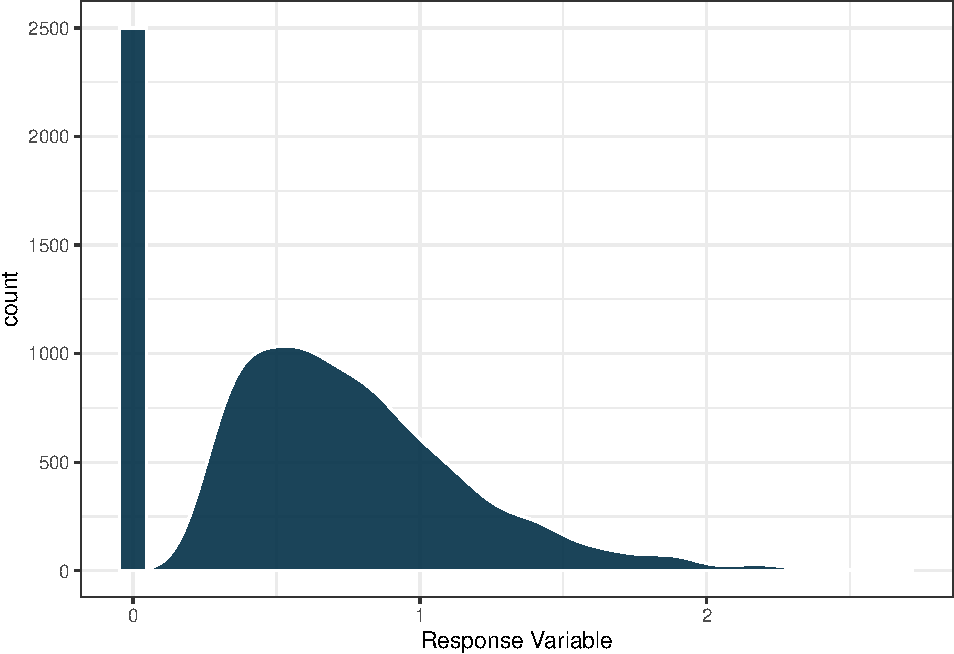
\includegraphics[width=0.85\linewidth]{thesis_files/figure-latex/ziex-1} 

}

\caption{Zero-Inflated data}\label{fig:ziex}
\end{figure}
And in reality, this form of zero-inflated data is one that we see quite often in the real world. Importantly, an abundance of zeros in a measured variable might come about for a variety of different reasons. Sometimes it could be a characteristic of the data itself, for example if we collected data on the total weight of fish caught at a lake by individuals on a given day, we likely would see a lot of individuals who caught zero fish leading to a significant portion of zeros in our data. But other times it could be a characteristic of the data collection process itself, for example a measurement error or a sampling error could cause data to be zero-inflated as well.

Importantly, as I am working in a modeling setting, \emph{when I say that data is zero-inflated I mean that the response variable is zero-inflated}. Although I will simply refer to my data as being zero-inflated and my models as being suited for zero-inflated data for the duration of this thesis, this is simply a matter of convenience and not a statement that the methods work for any situation in which data can be considered zero-inflated. Put simply, \emph{I explore, present, and evaluate a model that is suited for a response variable which has a significant portion of zeroes, with the non-zero portion of that variable belonging to a positive continuous distribution.}

\hypertarget{clustered-data}{%
\section{Clustered Data}\label{clustered-data}}

Furthermore, we will be operating in a setting where the data is not only zero-inflated, but where it also exhibits a clustered structure. Again, the notion of data being clustered is a very non precise one. For this thesis we will not put a very strong restriction on what this looks like. Our data will be clustered in the sense that there is meaningful grouping in the data structure that makes data points within the same cluster more alike on average than points across clusters.

For example, going back to the fishing in a lake example. If we looked at data on the weight of each individual fish caught, we would imagine that fish of the same species would generally be more similar in weight than two fish from different species.

\hypertarget{forestry-setting}{%
\section{Forestry Setting}\label{forestry-setting}}

One specific setting that exhibits both of these data features is data on the United States' forests. In particular, I will focus on forestry data collected by the Forestry Inventory \& Analysis Program (FIA) of the U.S. Government. The FIA monitors the nation's forests by collecting data on, and providing estimates for, a wide array of forest attributes. Not only is this work vitally important, but it's essential that it be done accurately and efficiently: ``The FIA is responsible for reporting on dozens, if not hundreds, of forest attributes relating to merchantable timber and other wood products, fuels and potential fire hazard, condition of wildlife habitats, risk associated with fire, insects or disease, biomass, carbon storage, forest health, and other general characteristics of forest ecosystems.''(McConville, Moisen, \& Frescino, 2020).

These sampled locations are referred to as plot-level data and the FIA sends a crew out to physically measure a wealth of forest attributes at that location. As you might expect, not only is this method extremely time intensive, but it is also very expensive. The vastness of the nation's forests in tandem with the resources needed to collect plot-level data, make it impossible to collect census level data on forest metrics. Thus, the need for additional data sources as well as statistical models are vital to the work that the FIA does. The main secondary data source that the FIA employes is remote sensed data. The remote sensed data typically includes climate metrics (e.g.~temperature and precipitation), geomorphological measures (e.g.~elevation and eastness), as well as metrics like tree canopy cover which can be measured from a satellite.

While the main use of the additional remote sensed data sources are to increase the accuracy of the estimators that the FIA builds, they are also used to make rational decisions about the aforementioned plot-level data collection. Before sending a crew out to a given sampled location, the FIA will first look at the remote sensed data for that location. If that location happens to be in a place where there is clearly no forest, for example in the middle of a parking lot, the FIA will not send a crew out and instead will mark all forest attributes for that location as being zero. As you might imagine, this happens quite a bit, and so an interesting characteristic of many forest attribute variables collected by the FIA is that they are zero-inflated. Importantly, this is an example of where the data is zero-inflated because of the data collection process.

Importantly, the FIA groups the continental U.S. into smaller domains called Eco-Subsections. These Eco-Subsections are drawn with the goal of maintaining internal ecologically homogeneity as best as possible. Thus each data point belongs to a specific Eco-Subsection and it's this grouping that gives us a clustered data structure.

If we look at the distribution of the FIA collected forest attribute ``Dry Above Ground Biomass From live Trees'', we can see that it is indeed quite zero-inflated.
\begin{figure}

{\centering 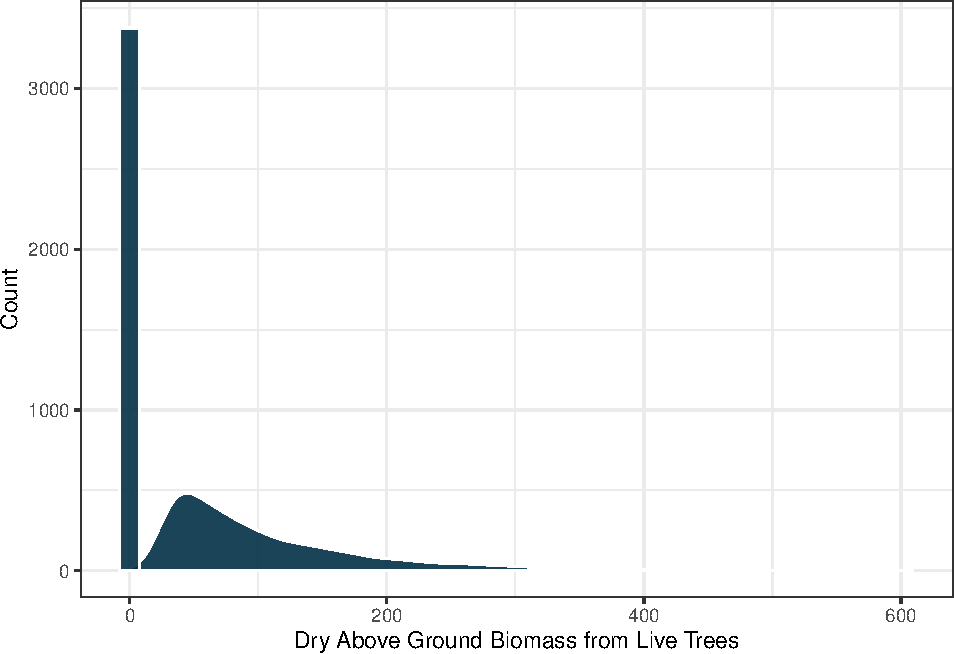
\includegraphics[width=0.8\linewidth]{thesis_files/figure-latex/forestrydata-1} 

}

\caption{Zero-Inflated Forestry data.}\label{fig:forestrydata}
\end{figure}
Not only is the FIA data a good real life example of when we see this zero-inflated and clustered data structure, but it's also a setting in which it's quite important that the models used to estimate these forest attributes are sufficiently accurate and efficient.

\hypertarget{immediate-modeling-struggles}{%
\subsection{Immediate Modeling Struggles}\label{immediate-modeling-struggles}}

To motivate using a more complex method, I'll first show what happens when I try to just fit a simple linear regression to this type of data. If we regress our response variable on a useful covariate and plot both the data and the simple linear regression line together we get the following
\begin{figure}

{\centering 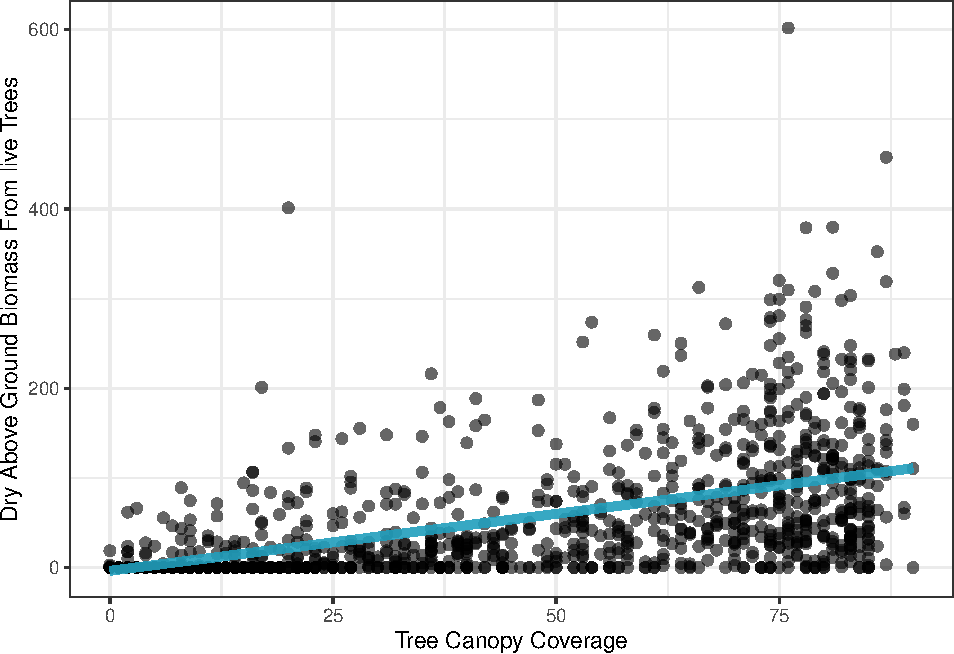
\includegraphics[width=0.8\linewidth]{thesis_files/figure-latex/scatterzi-1} 

}

\caption{The shortcomings of a simple linear regression model in this context.}\label{fig:scatterzi}
\end{figure}
While this model isn't awful it's certainly misspecified. What I mean by this is that a simple straight line shown in Figure \ref{fig:scatterzi} doesn't appropriately capture the dynamics of the relationship between our covariate and our response. The zero-inflation in the response variable pulls the regression line down so that it doesn't properly capture the relationship between the explanatory variable and the \emph{non-zero} response, but more importantly it doesn't capture the structure of zeros in the response at all. We can see that the only time this model will predict a near zero response is when the covariate value is very close to zero, but this is an extreme limitation of the model since we observe zero response values across almost the entire range observed values for the covariate. What's more, a simple linear regression model does not allow us to understand how the probability our response variable being zero, changes with our covariate.

We would call this model statistically biased, as it is overly simple and thus doesn't properly capture the structure of the data. While it's perhaps feels unfair to motivate my method by piting it against the simplest of statistical models, the reality is that linear regression is a very powerful and widely used model. Moreover, in a setting such as this one where the data looks plausibly linear, the principle of parsimony might make a linear regression model a well reasoned choice. While there's certainly a need for a model that is better fit to the data, I won't go down the route of constructing an incredibly opaque and complex deep learning model to do so. Instead they model I present is interpretable and intuitive while being flexible enough to capture the structure of the zero-inflated data.

\hypertarget{the-new-model}{%
\subsection{The New Model}\label{the-new-model}}

While I will exhaustively describe details of, and the math behind, the exact model in a later section, I'll go through a non-technical overview of how it will function here.

The defining characteristic of the model is that it is a two-part model. Instead of trying to fit the data with a singular model, we instead fit two different models and then combine them at the end. The two models are
\begin{enumerate}
\def\labelenumi{\arabic{enumi}.}
\item
  A classification model fit to the entire data set that predicts how likely it is that a certain data point has a non-zero response value.
\item
  A regression model fit to the \emph{non-zero} portion of the dataset that predicts the continuous response variable.
\end{enumerate}
To get a final prediction for a data point we take the prediction from model (1) and multiply it by the prediction from model (2).

\[
\text{Final Prediction} = \underbrace{\bigg(\text{Regression Model Output}\bigg)}_{\text{Model (2)}} \times \underbrace{\bigg(\text{Classification Model Output}\bigg)}_{\text{Model (1)}}
\]

Let's think back to Figure \ref{fig:scatterzi} to unpack why this is a reasonable strategy.
\begin{figure}

{\centering 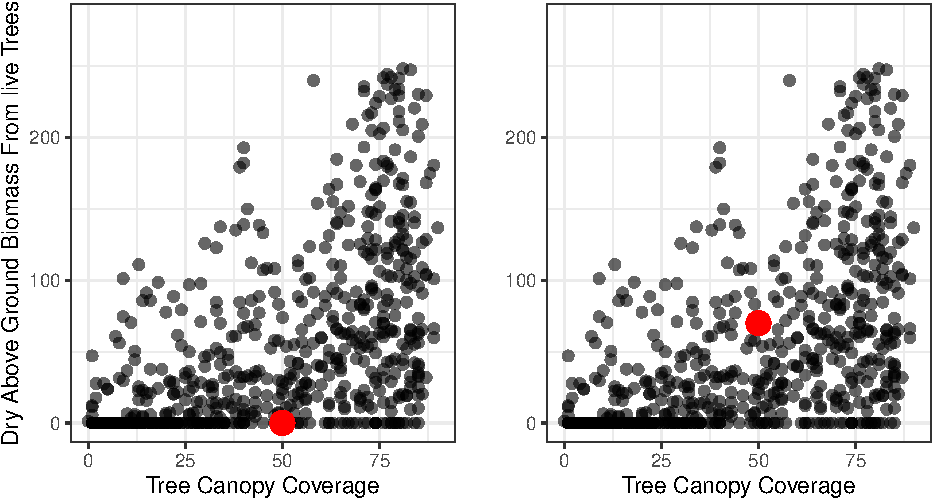
\includegraphics[width=0.95\linewidth]{thesis_files/figure-latex/modintuition-1} 

}

\caption{Example of two new data points that we might be interested in testing our model on.}\label{fig:modintuition}
\end{figure}
Let's start with the left hand side of Figure \ref{fig:modintuition} that has a data point with zero response value. We'd expect a very bad prediction from model (2) which was only fit to the non-zero data, but the intuition here is that if our classification model is sufficiently accurate then it shouldn't matter, as it will identify the point as being zero and thus the prediction will just be sent to zero by that classification model output.

On the other hand, the right hand side of Figure \ref{fig:modintuition} has a data point with non-zero response value. We'd expect a good prediction from model (2) here and again if the classification model is sufficiently accurate then it should identify it as being a non-zero data point and the model (2) prediction should be relatively unchanged when multiplied by the classification model output.

Clearly the success of this strategy relies on the quality of the two individual models, but at least we can see how this method has the capacity to capture the zero-inflation data structure.

\hypertarget{building-the-model}{%
\subsection{Building the Model}\label{building-the-model}}

Now, as the title suggests I'll be building these models in a Bayesian frame. But what does that even mean and why would one want to do that? While most of the thesis will be devoted to answering the second question, I'll spend some time in the next section describing Bayesian methods, and walking through how they differ from a Frequentist approach.

Importantly, since this thesis is simply an earnest exploration of a Bayesian method, it has no intention to participate in the deep and opaque philosophical dialogue regarding whether Bayesian or Frequentist methods are a more ``correct'' way to do statistics.

That being said, the word Bayesian is so overwhelmingly ideologically tied to this statistical dichotomy that it is, by nature, very difficult to talk about a Bayesian method without talking about Frequentism as well. Because classical statistical methods are all Frequentist ones, there is often a pressure to validate a Bayesian method by standing it next to its Frequentist counterpart. While this Bayesian thesis will indeed feature an alternative Frequentist method, it does so, not to argue for one side or the other, but rather to illustrate some of the key differences in, and logic behind, Bayesian and Frequentist analyses.

\hypertarget{looking-ahead}{%
\section{Looking Ahead}\label{looking-ahead}}

In order to introduce, study, and implement these models I will structure the research in the following way:
\begin{itemize}
\item
  Chapter \ref{bayes-freq} gives a thorough functional overview of how Bayesian and Frequentist methods differ in the simple setting of inference for a mean. The goal here is primarily to provide a gentle introduction to Bayesian data analysis, so as not to drop the reader into the deep end when the main model is introduced.
\item
  Chapter \ref{methods-sec} gives a detailed overview of all the methods employed in the thesis. It starts with a high-level description of the Zero-Inflation model, before moving on to detailed descriptions of how each model will be built. Next, prediction for Bayesian models is illustrated both theoretically and computationally. Finally, a mathematical proof is presented to justify building each part of the Bayesian two part model separately.
\item
  Chapter \ref{sim-study} sets up the simulation study that serves as the main process by which we evaluate the various models.
\item
  Chapter \ref{res-sec} showcases the results of each model's performance. Beyond comparing the performance metrics of each model, I also describe the challenges associated with making comparisons between Bayesian and Frequentist models in a complex setting like this one.
\item
  Chapter 6 gives an overview of the R Package written to accompany the methods explored in this thesis. A vignette is provided the applies the R Package to the Forestry data setting.
\end{itemize}
\hypertarget{bayes-freq}{%
\chapter{Frequentists and Bayesians}\label{bayes-freq}}

\hypertarget{bayesian-v.s.-frequentist-cryptic-definitions}{%
\section{Bayesian ``v.s.'' Frequentist: Cryptic Definitions}\label{bayesian-v.s.-frequentist-cryptic-definitions}}

Perhaps the biggest roadblock for understanding how a Bayesian methodology differs from a Frequentist one stems from the fact that most of the statements you find on the internet are short cryptic quips that, while true, are largely unhelpful for someone just starting to dig in.

For example, a simple Google search for ``Bayesian v.s. Frequentist'' will tell you that this statistical philosophic divide is mainly a question of what we mean by probability. The top search result will likely say that for Frequentists, probabilities are fundamentally related to the frequencies of repeated events, while for Bayesians probabilities are related to one's own certainy or uncertainty about events. Again, while this statement is correct and does lead to many of the main functional differences between the two methods, it's nearly impossible to translate this statement into an understanding of how the methods differ in practice.

If you dig a bit deeper and refine your Google search, you'll eventually come across a more technical definition such as this one from Gelman:
\begin{quote}
``Bayesian statistical conclusions about a parameter \(\theta\) are made in terms of probability statements. These probability statements are conditional on the observed value of {[}x{]}, and \ldots{} are written simply as \(p(\theta \ | \ x)\) \ldots{} It is at the fundamental level of conditioning on observed data that Bayesian inference departs from the approach to statistical inference described in many textbooks, which is based on a retrospective evaluation of the procedure used to estimate \(\theta\) over the distribution of possible {[}x{]} values conditional on the true unknown value of \(\theta\)'' \footnote{Gelman, Carlin, Stern, \& Rubin (1995)}
\end{quote}
It's not important to understand what this is saying right now, but I include it here because in just a few sentences Gelman fully lays out the core difference between Bayesian and Frequentist methods. While it is not a good entry point for someone just beginning to learn, it will be helpful to return back to portions of this excerpt as we work through an extended example.

\hypertarget{worked-example-a-better-way-to-learn}{%
\section{Worked Example: A better way to learn}\label{worked-example-a-better-way-to-learn}}

At a very high level, the fact that one should always return to when comparing a Bayesian and Frequentist methodology is that in an analysis for a parameter \(\theta\)
\begin{itemize}
\item
  Frequentists treat the observed data as random and the parameter as fixed. Thus they aim to quantify how the data might vary around the fixed (but unknown) parameter value.
\item
  Bayesians treat the observed data as fixed and the parameter as random. Thus they try to quantify how the parameter might vary based on the fixed observed data.
\end{itemize}
With this in mind, we now turn to a simple inference example.

Suppose we are interested in estimating the average weight of squirrels in a given park, let's call this \(\theta\). Moreover, suppose that we want to somehow quantify our uncertainty for that estimate. Suppose that the distribution of the weight for the entire squirrel population in that park is \(\mathcal{N}(\theta, 1)\) (we treat the standard deviation as being fixed and known so as to simplify our example) and that we've properly collected a random sample \(\{X_1, X_2, ..., X_n\}\) from the population.

\hypertarget{frequentist-version}{%
\subsection{Frequentist Version}\label{frequentist-version}}

We choose \(\bar{X}\) as our point estimate and because of the Central Limit Theorem we can say that it is distributed \(\mathcal{N}(\theta, 1/n)\). And indeed, as laid out above, by using asymptotic theory to place a distribution on the data, we are treating the data as random and the unknown parameter as fixed. Some shifting and scaling tells us that,

\[
\frac{\bar{X} - \theta}{1/\sqrt{n}} \sim \mathcal{N}(0,1)
\]

Furthermore, properties of the Normal distribution tell us that,

\[
\begin{aligned}
P\bigg(-1.96 < \frac{\bar{X} - \theta}{1/\sqrt{n}} < 1.96\bigg) = 0.95 \implies P\bigg(\bar{X} - 1.96\cdot\frac{1}{\sqrt{n}} < \theta < \bar{X} + 1.96\cdot\frac{1}{\sqrt{n}}\bigg) = 0.95
\end{aligned}
\]

So a Frequentist would end up with what is called a 95\% confidence interval for \(\theta\) of:
\begin{equation}
  \bigg(\bar{X} - 1.96\cdot\frac{1}{\sqrt{n}}, \ \bar{X} + 1.96\cdot\frac{1}{\sqrt{n}}\bigg)
  \label{eq:freq-ci}
\end{equation}
Let's pause to ask ourselves what is random in Equation \eqref{eq:freq-ci}. For starters, \(\bar{X}\) is certainly random since it came from a random sample from the population, but an immediate implication of this is that the interval itself is actually random too. The very first step in our process was to use asymptotic theory (the Central Limit Theorem) to place a distribution on our observed data \(\bar{X}\). This randomness in the data thus carries through to our confidence interval and we end up with an uncertainty statement about the \textbf{procedure} being performed and not the parameter itself. Different samples will results in different \(\bar{X}\)s which will result in different confidence intervals.

It's perhaps easiest to understand how to interpret Equation \eqref{eq:freq-ci} through a quick simulation and visualization. If we generated a 100 new samples from the population with the true parameter \(\theta\) being 5, and computed a confidence interval for each, we could then plot all 100 intervals and count how many of them contain the true parameter.
\begin{figure}

{\centering 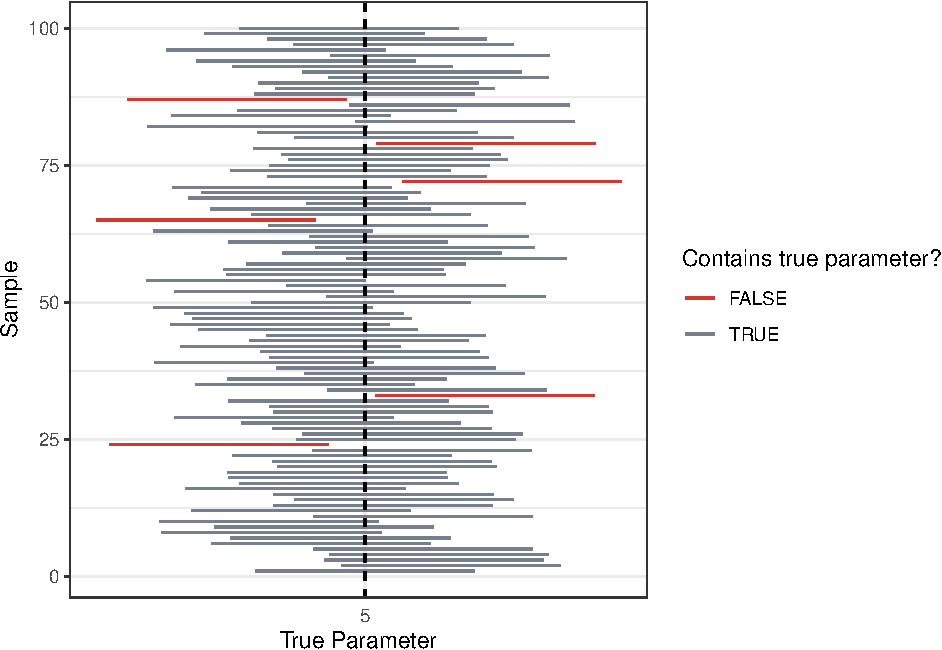
\includegraphics[width=0.8\linewidth]{thesis_files/figure-latex/ci-coverage-ex-1} 

}

\caption{A visualization of Frequentist confidence intervals.}\label{fig:ci-coverage-ex}
\end{figure}
First of all, \ref{fig:ci-coverage-ex} really drills home the point that Frequentists treat the parameter as fixed and try to quantify how the data might vary around it. Here we see that in 6 of our iterations of this sampling procedure, the confidence interval did not contain the true parameter, giving us coverage of 94\%. The reason we did not observe 95\% coverage, is again due to the fact that the intervals are random and Equation \eqref{eq:freq-ci} is an asymptotic statement about the process of resampling data and computing a new confidence interval. Thus, the correct interpretation of Equation \eqref{eq:freq-ci} is that if we repeated the sampling procedure many times, we'd expect the true mean, \(\theta\), to be captured by such an interval 95\% of the time.

With this new understanding, we can unpack why it's incorrect to interpret Equation \eqref{eq:freq-ci} as saying that ``the interval contains the true parameter with probability 0.95''. As we just saw, our confidence interval is really a statement about a result we'd see if we repeated the whole procedure many times, and it is absolutely not a statement about any singular instance of the procedure. For a given confidence interval, the true parameter either lies within the interval or it doesn't, with 100\% certainty.

\hypertarget{revisiting-the-cryptic-definitions}{%
\subsubsection{Revisiting the Cryptic Definitions}\label{revisiting-the-cryptic-definitions}}

Before moving on to exploring how a Bayesian would tackle this inference problem, think back to the beginning of the section where we described how an internet search might tell you that a Frequentists conceptualize probability in terms of frequency of related events. While this statement is largely unhelpful on it's own, it actually becomes quite helpful when taken together with the example that we've just walked through. Through a Frequentist lense, the probability statement in Equation \eqref{eq:freq-ci} must be conceptualized in terms of frequenct of related events, which in this case is hypothetical resampling of the data.

What's more, while it's still overly complicated in it's language, Gelman's statement that Frequentist inference is ``based on a retrospective evaluation of the procedure used to estimate \(\theta\) over the distribution of possible {[}x{]} values conditional on the true unknown value of \(\theta\)'' (Gelman et al., 1995), can at least partially be understood. Each of these pieces are things ideas that we've developed through our example:
\begin{itemize}
\tightlist
\item
  The retrospective evaluation of the procedure used to estimate \(\theta\): In the example this was the resampling of our data
\item
  over the distribution of possible {[}x{]} values: In our example this involved using the Central Limit Theorem to place a distribution on our data
\item
  conditional on the true unknown value of \(\theta\): Treating \(\theta\) as fixed but unknown.
\end{itemize}
While these definitions are still found to be lacking when trying to absorb them on their own, in the context of our example, we can start to understand and appreciate the things that they are saying.

\hypertarget{bayesian-version}{%
\subsection{Bayesian Version}\label{bayesian-version}}

Instead of first describing the nuts and bolts of how we estimate both the parameter of interest and the uncertainty in that estimate as we did in the previous section, we start at the end with the final expression for both of these things in order to draw some of the most important similarities and differences between the two methods.

\hypertarget{general-form}{%
\subsubsection{General Form}\label{general-form}}

A good place to start whenever performing a Bayesian analysis is to remember that ``the guiding principle for bayesian statistics is that the state of knowledge about anything unknown is described by a probability distribution.'' (Gelman et al., 1995). In the context of inference where we're interested in an unknown parameter \(\theta\), a Bayesian describes all of their knowledge about \(\theta\) using a probability distribution. In particular, Bayesians use a specific distribution to do so- the posterior distribution. The posterior distribution is the center of interest for all Bayesian analyses and it is simply the distribution of the parameter of interest, conditional on the fixed observed data: \(p(\theta \ | \ x)\).

Let's step back for a moment and think about what the immediate implications of this framework are. By describing our knowledge about \(\theta\) using a distribution we are already doing something very different form in the Frequentist version. Here we are treating our observed data as fixed and our parameter of interest as random. In particular, we make conclusions about the distribution of \(\theta\), a.k.a how it varies, conditional on our observed data which we treat as fixed. For a Bayesian, this distribution holds all of the available information about \(\theta\) and thus is the focus of their attention. So in the context of our example, when a Bayesian wants to perform inference for the mean weight of squirrels in a park, they will do so by constructing a posterior distribution that describes how the \emph{true} mean weight might vary conditional on the fixed observed data.

Once we have an expression for out posterior, we quantify our uncertainty by creating what are called credible intervals. We do so by finding an interval \(C\) such that,

\[
\int_C p(\theta \ | \ x)d\theta = 0.95
\]

Again, notice how drastically this differs from the Frequentist calculation of an uncertainty estimate. No longer do we rely on asymptotic theory about the randomness of the data sampling process, but instead, since we treat the parameter as random, our uncertainty pertains to the fact that we have uncertainty about what that true parameter is. While estimation of the parameter and uncertainty in that estimate is a two step process in the Frequentist framework (first calculate \(\bar{X}\), then use theory to calculate the confidence interval), both things are baked right into the posterior distribution in the Bayesian framework. This is by far one of the most appealing aspects of using a Bayesian method: because we make conclusions in terms of probability statements, we get uncertainty estimates ``at no extra cost'' in all of our analyses. While increasingly complex Frequentist methods might require increasingly complex procedures for estimating uncertainty, a Bayesian model can be expanded in complexity with no extra work required to acquire uncertainty estimates.

Furthermore, once we compute C, then we can correctly say that.
\begin{equation}
  P(\theta \in C \ | \ x) = 0.95
  \label{eq:bayes-ci}
\end{equation}
And here we really do mean that the probability that our interval \(C\) captures \(\theta\) is 0.95. \textbf{Bayesians conceptualize probability in terms of certainty, or uncertainty, about events, meaning that their probability statements can be about the unknown parameter itself}.

\hypertarget{back-to-the-cryptic-definitions}{%
\subsubsection{Back to the Cryptic Definitions!}\label{back-to-the-cryptic-definitions}}

Again, it's the fact that Bayesians conceptualize probability as being related to one's own certainy or uncertainty, that allows us to interpret \eqref{eq:bayes-ci} in the way that we do. Furthermore, if we revisit Gelman's quote as well that ``Bayesian statistical conclusions about a parameter \(\theta\) are made in terms of probability statements. These probability statements are conditional on the observed value of {[}x{]}, and \ldots{} are written simply as \(p(\theta \ | \ x)\)''\footnote{Gelman et al. (1995)}, we can directly tie it into what we showed above.

Now that we've explained the gist of Bayesian analysis at a high level, we'll dive into the nuts and bolts of how the posterior is actually computed.

\hypertarget{building-an-estimate}{%
\subsubsection{Building an Estimate}\label{building-an-estimate}}

So how do we actually calculate and estimate \(p(\theta \ | \ x)\)? As the name of the framework suggests, we leverage Bayes Theorem as a way to try to quanitfy the posterior distribution. Bayes Theorem tells us that we can break it down into three separate pieces.

\[
p(\theta \ | \ x) =  \frac{p(x \ | \ \theta)p(\theta)}{p(x)}
\]

So the problem of quantifying \(p(\theta \ | \ x)\) is really a problem of quantifying these three other pieces. Traditionally \(p(x \ | \ \theta)\) is referred to as the likelihood function, which is treated as being a function of \(\theta\), and we can think of it capturing how likely it would be for us to observe the sample data \(x\) given a certain realization of \(\theta\). Next, \(p(\theta)\) describes our belief about \(\theta\) \emph{before} we have performed any analysis, and thus it is aptly named the prior. \(p(x)\) is just a function of the data and thus is referred to as, and treated like, a normalizing constant. Because of this we usually just ignore it and write,

\[
p(\theta \ | \ x) \propto p(x \ | \ \theta)p(\theta)
\]

In plain English, we can imagine a Bayesian approach progressing in the following way. First we supply a prior belief about the unknown parameter. Then, once we observe the data we can generate an expression for the likelihood and can update our belief by multiplying our prior by that likelihood to get our posterior \(p(\theta \ | \ x)\).

Importantly, while the likelihood function, \(p(x \ | \ \theta)\), is a function of \(\theta\), it comes directly from the data, meaning that there isn't any flexibility in how we represent that term. But perhaps the largest, and most contentious, consequence of describing \(\theta\) by a probability distribution conditioned on \(x\) is that Bayes Theorem forces us to supply a prior distribution \(p(\theta)\) ourselves. The reality is that Bayes theorem places almost no restrictions on what \(p(\theta)\) could be and this means that in certain cases, drastically different priors can lead to very different posterior distributions. There is a whole body of literature that talks about this ``subjective'' aspect of a Bayesian analysis, but as we will show later in this thesis, these priors can actually be very powerful in their ability to regularize our analysis. If we have some prior information about \(\theta\) it makes sense to try to utilize it, and the prior distribution gives us a way to do so.

To clear up what all of this looks like in practice, we'll now walk through our squirrel weights example in this Bayesian setting. As we walk through this process, just remember that at the end of the day, all we're really doing is choosing a prior, computing the likelihood, and multiplying the prior by the likelihood.

We might start by guessing that squirrels might weight around 1.5 pounds on average, and attach a relatively large variance to that guess of 10. So the prior that we supply could be \(f(\theta) = \mathcal{N}(1.5,10)\). While there is a huge literature on how you should choose your priors, for now, all you need to know is that at the very least a prior should extend over the entire range of possible values that your unknown parameter could take on. While we could use a distribution that was strictly positive to emphasize the fact that \(\theta\) is certainly positive, we'll stick with a normally distributed prior for the sake of simplicity (in fact what makes this a simple choice is that it achieves something called conjugacy which in this case just means that it guarantees that our posterior will also be a normal distribution).

Next we use Bayes Theorem to combine our prior with the observed data:

\[
\begin{aligned}
p(\theta \ | \ x) &\propto \mathcal{L}(\theta \ | \ x)p(\theta) \\
&= \bigg[\prod_{i=1}^n\mathcal{L}(\theta \ | \ x_i)\bigg]p(\theta) \\
&= \bigg[\prod_{i=1}^n\frac{1}{\sqrt{2\pi}}\text{exp}\bigg(-\frac{1}{2}(x_i - \theta )^2\bigg)\bigg]\frac{1}{\sqrt{2\pi\cdot10^2}}\text{exp}\bigg(-\frac{1}{2\cdot10^2}(\theta - 1.5)^2\bigg) 
\end{aligned}
\]

a rather large amount of math will simplify this down to

\[
p(\theta \ | \ x) \propto \frac{1}{\sqrt{2\pi\sigma_f^2}}\text{exp}\bigg(-\frac{1}{2\sigma_f^2}(\theta - \theta_f)^2\bigg)
\]

Which we can recognize as being a normal distribution with mean \(\theta_f\) and variance \(\sigma^2_f\) . In particular \(\theta_f\) and \(\sigma^2_f\) are

\[
\begin{aligned}
\theta_f &= \frac{\frac{1}{10^2}\cdot1.5 + n\cdot \bar{x}}{\frac{1}{10^2} + n} \\
\sigma^2_f &= \frac{10^2}{1 + 10^2\cdot n}
\end{aligned}
\]

where each have notably been influenced by both the prior and the likelihood. It can be helpful to visualize what has happened here with a plot.
\begin{figure}

{\centering 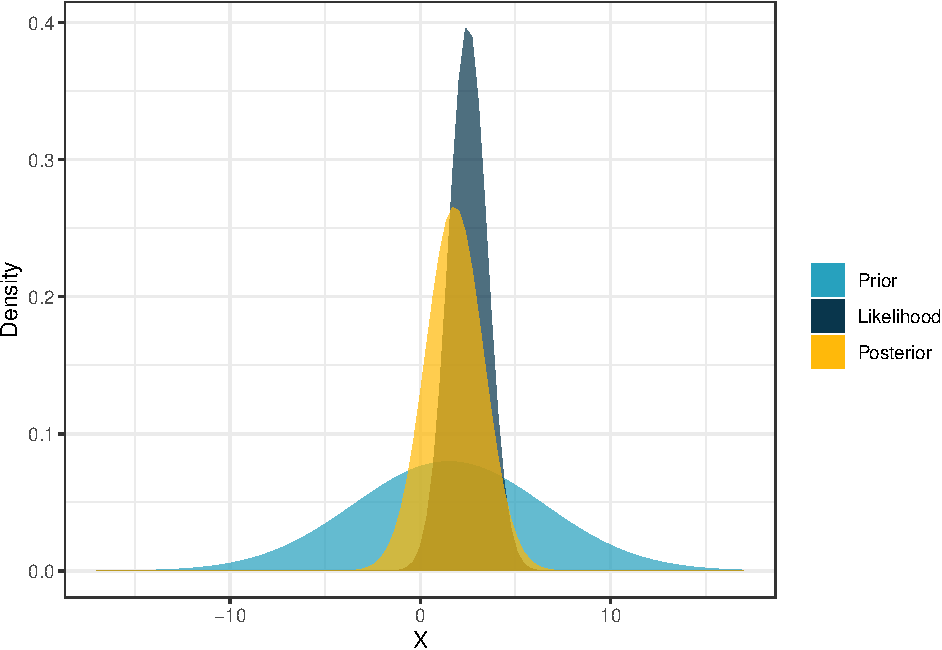
\includegraphics[width=0.8\linewidth]{thesis_files/figure-latex/bayes-dists-1} 

}

\caption{The Prior, Likelihood, and Posterior for this example all plotted together.}\label{fig:bayes-dists}
\end{figure}
Above we see the three main components of a Bayesian analysis plotted all together. It's helpful to visualize what's happening here because it really drills home the idea that the posterior is, in a sense, a tradeoff between the prior and the likelihood function. More technically, the posterior is the normalized product of the likelihood and the prior. The result is that the prior information has pulled the posterior to the left and has introduced more variance than from the likelihood function alone.

Clearly, even in this simple example it takes quite a bit of work to derive the exact expression for the posterior. In fact, in practice the posterior is often times something that is incredibly complicated and so we don't even bother trying to simplify the product of the likelihood and the prior down into a distribution that we can recognize. Instead we make use of the massive computational advances that have been made that allow us to algorithmically approximate the posterior. Mainly, a process called Markov Chain Monte Carlo (MCMC) is used due to it's very powerful ability to produce samples from the posterior distribution.

\hypertarget{takeaways}{%
\section{Takeaways}\label{takeaways}}

In summary, in a Frequentist analysis the question being asked is ``What sort of \(\hat{\theta}\) would we expect to get under hypothetical resampling?'', while in a Bayesian analysis the question is ``What is our knowledge of \(\theta\) based on the data and our prior information?''

While this thesis will focus on statistical predictive models rather than inference, the fundamental functional differences remain the same. To build a model in a Bayesian frame is to represent one's knowledge about the model parameters using probability distributions. What's more, predictions are no longer point estimates but rather distributions themselves. As stated earlier, \emph{the state of knowledge about anything unknown is described by a probability distribution}.

This all seems fine and interesting, but at the end of the day the question remains- why bother doing statistical analysis in this way? This thesis should be read as a log of the time I spent trying to answer that question and not as some strongly opinionated piece about the quality of Bayesianism relative to Frequentism.

\hypertarget{methods-sec}{%
\chapter{Methods}\label{methods-sec}}

We now move into a thorough description of all of the methods employed in this thesis. In subsections \ref{notation}-\ref{specificmods} the necessary notation and model structure are introduced. While the rest of the subsections intermittently mention the Frequentist model, they are primarily focused on the Bayesian models. In particilar, \ref{twofits} describes how the Bayesian models are fit, \ref{bayespred} describes what prediction with a Bayesian model looks like, \ref{sepsim} presents a theoretical backing for why the components of the Bayesian two-part model can be fit separately, and finally \ref{wrapone} and \ref{wraptwo} wrap everything up.

\hypertarget{notation}{%
\section{Notation}\label{notation}}

Let \(U\) denote a finite population with \(N\) elements. \(U\) is broken into \(J\) groups \(U_j\), \(j = 1, 2, ..., J\), where each group \(U_j\) is defined as having \(n_j\) sample observations. Let \(p = 1, ..., P\) index the covariates. Each sample observation, \(i\) in group \(j\) has auxiliary information \(x_{ij}^p\) for covariate \(p\), response value \(y_{ij}\), and indicator for being non-zero \(z_{ij}\).

\[
z_{ij} =
\begin{cases}
1 & \text{if}\ \ y_{ij} \ne 0 \\
0 & \text{if} \ \ y_{ij} = 0
\end{cases}
\]

\hypertarget{model-structure-formalized}{%
\section{Model Structure Formalized}\label{model-structure-formalized}}

We now introduce the modeling technique that will be the main focus of the thesis. Wonderfully, there is some real mathematical backing for why we might build this model in the way that we do, and I think that looking at the steps draws out a lot of helpful intuition.

Let \(Y\) represent the response variable and \(X\) represent the covariates. We typically write \(\mathbb{E}[Y \ | \ X]\) to denote the expected value of our response variable conditional on it's covariates. Since the separation of the response into values that are zero and those that are not is a finite partition, we can leverage the law of iterated expectation to expand our model structure:
\begin{equation}
\begin{split}
    E[ Y  \ | \ X = x] &= \underbrace{E[Y \ | \ X = x, Y = 0]}_{= \ 0}P(Y = 0 \ | \ X = x) + E[Y \ | \ X = x, \ Y > 0]P(Y> 0 \ | \ X = x) \\
    &= E[Y \ | \ X = x, \ Y > 0]P(Y > 0 \ | \ X = x) 
\end{split}
\label{eq:intuition}
\end{equation}
Out of this equation comes a wonderful intuition for what our new modeling process will look like, what we end up with is something that is somewhat meta in that it doesn't tell us what the exact model will be, but rather it tells us what the structure of our model should look like. What we do know is that we should have one model that predicts our non-zero response using our covariates \(E[Y \ | \ X = x, \ Y>0]\), and another that predicts whether our response is non-zero or not, again using the covariates \(P(Y > 0 \ | \ X = x)\).

Think back to the Introduction where we introduced the model as being:

\[
\text{Final Prediction} = \bigg(\text{Regression Model Output}\bigg) \times \bigg(\text{Classification Model Output}\bigg)
\]

all we've done above is provided a formal theoretical backing for this structure and strategy.

Importantly, while Equation \eqref{eq:intuition} describes the broader two-part model strategy that will be employed by both the Frequentist and Bayesian versions of the model, the formulation can't technically be extended into the context of prediction for the Bayesian model. Equation \eqref{eq:intuition} does describe how prediction functions in the Frequentist case, but as we will get to later in the Bayesian setting everything is described by a probability distribution and so we aren't working with expected values anymore. That being said, this is just a small technicality that shouldn't take away from the really nice larger intuition that Equation \eqref{eq:intuition} holds for both models.

\hypertarget{specificmods}{%
\section{Specific Models}\label{specificmods}}

Although we could model these two parts however we wanted to, we will use a generalized linear regression model (that is non-logistic) for the first part and a logistic regression model for the second. Moreover, because the data we will be working with has a clustered structure we attempt to capture that by including group-level random effects in both models. The precise models that we will be evaluating will be as follows.

We fit a generalized linear model with random intercepts to the \textbf{non-zero} portion of the data (the \(*\) helps differentiate this model from our final model). The linear predictor is specified as follows

\[
\mu_{ij} = \mathbf{x}_{ij}^T\boldsymbol{\beta} + u_j + \varepsilon_{ij} \qquad \text{where} \qquad u_j \sim \mathcal{N}(0, \sigma_{u}^2)
\]

With a link function \(g^{-1}\) and a probability distribution for the response, we get the final model as

\[
y^*_{ij} = g^{-1}(\mu_{ij})
\]

At this point we don't place a specific distributional assumption on the error term \(\varepsilon_{ij}\) because this will vary with the specific generalized linear model being employed. To spoil the surprise, the two GLMs that we will look at will be one with identity link and Normal distribution (i.e normal linear regression), and one with the log link and a Gamma distribution. That being said, we keep the notation broad at this point so as to emphasize the fact that this portion of the model aims to capture the structure of the non-zero response, and even though we try to model it using various distributions, this is still the main goal.

Here, \(\mathbf{x}_{ij}^T = (x^1_{ij}, ..., x^P_{ij})\) is a \(P\times 1\) vector of covariates, \(\boldsymbol{\beta}\) is a \(1\times P\) vector of fixed effects, and \(u_j\) is the random effect associated with group \(j\). Finally, \(\sigma^2_{u}\) is the between group variance parameter. The distribution on \(\varepsilon_{ij}\) will change depending on the specifics of the glm that we employ.

Next we fit a logistic regression random intercepts model to the full data set

\[
P(z_{ij} = 1) = p_{ij} = \frac{1}{1 + e^{-(\mathbf{x}_{ij}^T\boldsymbol{\gamma} + v_j)}} \qquad \text{where} \qquad v_j \sim \mathcal{N}(0, \sigma_{v}^2)
\]

Here \(\boldsymbol{\gamma}\) is a \(1\times P\) vector of fixed effects and \(v_j\) is the random effect associated with group \(j\). Again, \(\sigma^2_{v}\) is the between group variance parameter.

We will get into how each of these model pieces are estimated in the next section, but once we have estimates for all of our coefficients, we get our final model by taking the product of these two estimated models.

\[
\hat{y}_{ij} = \hat{y}^*_{ij}\cdot \hat{p}_{ij}
\]

And we get a prediction for a single group by averaging the predictions over all samples in that group.

\[
\hat{Y}_j = \frac{1}{n_j}\sum_{i \in n_j}\hat{y}^*_{ij}\cdot \hat{p}_{ij}
\]

Importantly, while \(y^*_{ij}\) is fit on only the non-zero data, and \(p_{ij}\) is fit on the entire data, when we make predictions on new data, both models are applied to the entire new data set.

\hypertarget{twofits}{%
\section{Model Fitting: Two Ways}\label{twofits}}

\hypertarget{frequentist}{%
\subsection{Frequentist}\label{frequentist}}

As it is not the focus of this thesis, we will not go in depth into how these models are fit in a Frequentist setting. Still, it's important to at least provide a brief summary of how it is most often done.

In most cases (and in particular in most statistical software), Frequentist regression models are fit using something called Maximum Likelihood Estimation (MLE). Very broadly, MLE functions by first assuming that the observed data was sampled from some distribution. Out of that assumption we get a likelihood function \(p(\text{data} \ | \ \text{parameters})\). And finally, as the name suggests, we choose parameter values that maximize the likelihood of the observed data given that parameter. The main gist of what's happening here is that we are answering the question: under what fixed parameter values would we be most likely to see the data that we observed? In the case of a statistical model this translates into: what parameter values maximize the likelihood that the process described by the model produced the data that were actually observed?

We won't say much more about this process and this strategy other than to tie it back to some of the ideas laid out in Section \ref{bayes-freq}. By making an assumption about the model that best describes the process that generated the data, we are conceptualizing the data as being random. The goal is to figure out which fixed parameters define a process that would have been most likely to produce an instance of the data like the one we observed.

\hypertarget{bayesian}{%
\subsection{Bayesian}\label{bayesian}}

Before diving into the specifics of the Bayesian model fitting, recall that a Bayesian analysis proceeds by treating the data as fixed and the unknown parameters as random. Importantly we still are interested in estimating the posterior \(p(\theta \ | \ \text{data})\), but now we have many parameters of interest \(p(\beta_1, \beta_2, \sigma^2_{u}, ... \ \text{etc} \ | \ \text{data})\), and so the expressions get a bit more complicated. As we get into all of the specifics that we lay out below, always remember that at the core of this process, we aree= treating our parameters as random and trying to quantify how they might vary given our fixed data.

We'll start by describing the logistic regression model, before moving on to the two different versions of the generalized linear regression component.

\hypertarget{logistic-regression-component}{%
\subsubsection{Logistic Regression Component}\label{logistic-regression-component}}

Again we start by specifying the broad distribution of our response in this model

\[
z_{ij} \sim \text{Bernoulli}\Bigg(\frac{1}{1 + e^{-\mu_{ij}}}\Bigg) \qquad \text{where} \qquad \mu_{ij} =\mathbf{x}_{ij}^T\boldsymbol{\gamma} + v_j
\]

So far we have done nothing differently than in the usual frequentist formulation of a model, but now instead of treating our model parameters as fixed but unknown, we treat them as random variables and attach priors to them. The random intercepts are given a normal prior centered on zero with hyper-prior \(\sigma_v^2\).

\[
v_j \ | \ \sigma_{v}^2 \sim \mathcal{N}(0, \sigma_{v}^2)
\]

Although \(\boldsymbol{\gamma}\) and \(\sigma_{v}^2\) are different parameters than the one's in the previous model, we attach the same priors to them

\[
\begin{aligned}
\gamma_p &\sim \mathcal{N}(m_p, s_p^2)  \qquad \forall p\in 1...P \\
\sigma_{v}^2 &\sim \text{Half-Cauchy}(0, r_1^2)
\end{aligned}
\]

The prior parameters \(m_p, s_p^2, r_1^2\) are real-valued numbers that center and scale the priors, thus they are chosen with the specifics of the data set in mind. A Half-Cauchy distribution is just a Cauchy distribution bounded to non-negative values, and is broadly utilized as a prior for variance parameters due to the fact that ``even in the tail, they have a gentle slope (unlike, for example, a half-normal distribution) and can let the data dominate if the likelihood is strong in that region.''\footnote{Gelman (2006)}. While dependence between priors \emph{can} be modeled in a bayesian frame, we will assume that all of our priors are independent of each other.

An example of what the prior distributions look like across a few of their parameter values is shown below.
\begin{figure}

{\centering 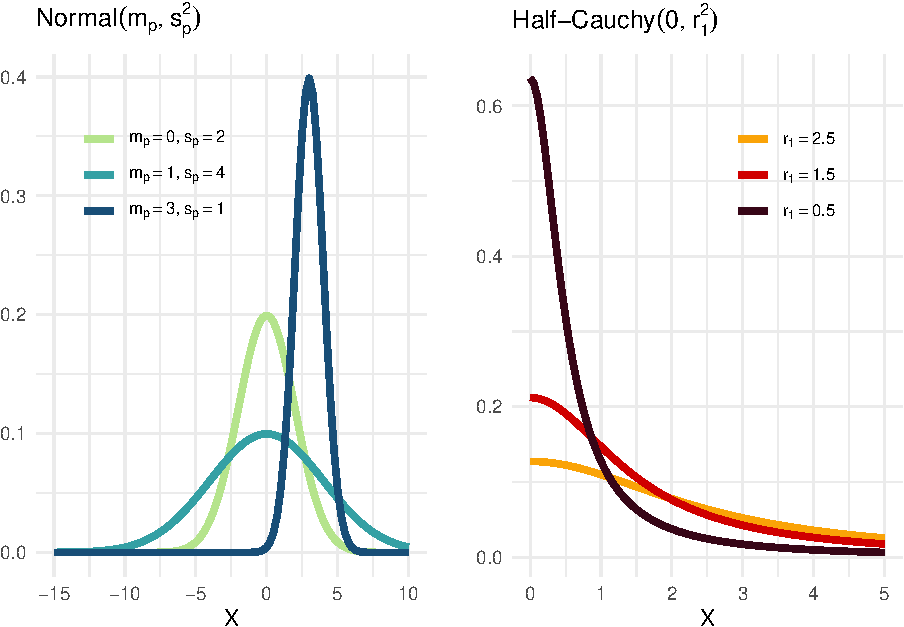
\includegraphics[width=0.8\linewidth]{thesis_files/figure-latex/priors-1} 

}

\caption{Various parameter values for the prior distributions.}\label{fig:priors}
\end{figure}
Again, in estimating the actual \textbf{model parameters} in a Bayesian analysis the goal is to recover the joint posterior distribution of those parameters. Let \(\boldsymbol{\gamma} = (\gamma_1, ...,\gamma_P)\) and \(\mathbf{v} = (v_1, ..., v_J)\). The joint posterior distribution can be written as

\[
\begin{aligned}
p(\boldsymbol{\gamma}, \mathbf{v},  \sigma_v^2 \ | \ \mathbf{y}) &\propto \bigg[\prod_{i=1}^np(y_i \ | \ \boldsymbol{\gamma}, \mathbf{v},  \sigma_v^2)\bigg]\cdot p(\gamma_1, ...\gamma_P, v_1,... ,v_J, \sigma_{v}^2) \\
 &= \bigg[\prod_{i=1}^np(y_i \ | \ \boldsymbol{\gamma}, \mathbf{v},  \sigma_{v}^2)\bigg]\cdot p(\gamma_1)\cdot...\cdot p(\gamma_P)p(v_1) \cdot ... \cdot p(v_J)p(\sigma_{v}^2)
\end{aligned}
\]

If we were able to compute a closed form expression for the posterior, we could then attain posteriors for each of our individual model parameters by marginalizing- i.e integrating out all of the other parameters. For example, we might be interested in the posterior of only \(\sigma_u^2\). In that case, the marginal posterior can be computed as follows:

\[
p(\sigma_{v}^2 \ | \ \mathbf{y}) = \int_{\gamma_1} \cdots \int_{\gamma_p} \int_{v_1} \dots \int_{v_J} p(\boldsymbol{\gamma}, \mathbf{v},  \sigma_{v}^2 \ | \ \mathbf{y}) d\beta_1 ... d\beta_P dv_1 ... dv_J
\]

The result would be a probability density function that encapsulates all of our information about \(\sigma_{v}^2\).

As it turns out, the models are often complex enough that the RHS will not result in a recognizable probability density function. Thus we employ a Markov Chain Monte Carlo (MCMC) algorithm to simulate draws from the approximate posterior. To do so we use the probabilistic programming language ``Stan''. The specific version of MCMC algorithm that Stan runs is called ``Hamiltonian Monte Carlo''. While this thesis will not describe MCMC in depth, the short and sweet description is that an MCMC algorithm's strategy for drawing samples from an unknown probability distribution is to wander around the space in such a way that the amount of time spent in each location is proportional to the height of that distribution. The real nuts and bolts of the algorithm lie in how decisions are made about how and where to move around in the space so that the result is obtained. The especially powerful thing about MCMC algorithms is that under enough iterations, they construct a Markov Chain (random walk) that \emph{has the desired posterior distribution as it's stationary distribution.} Thus we have to be a little bit careful with our language when interpreting the MCMC output. It's not that we are attaining samples from the actual posterior distribution (after all it is unknown), but rather stops along the random walk that is exploring the unknown posterior. That being said, if the MCMC algorithm converges properly then we will have samples from the approximate posterior distribution that should have characteristics similar to the actual posterior.

In it's most basic configuration Stan will output 2,000 sets of parameter draws which represent samples from the approximate joint posterior distribution.

\[
\begin{bmatrix}
  \gamma_1^{(1)} & \dots & \gamma_P^{(1)} & v_1^{(1)} & \dots & v_J^{(1)}  & (\sigma_{v}^2)^{(1)} \\
  \\ \vdots   &  & \vdots  & \vdots & &  \vdots & \vdots  \\ \\
  \gamma_1^{(2000)} & \dots &\gamma_P^{(2000)} & v_1^{(2000)}& \dots & v_J^{(2000)} & (\sigma_{v}^2)^{(2000)}
\end{bmatrix}
\]

One really nice aspect of this is that the while the combination of all of the columns in the output represent samples from the approximate \textbf{joint} posterior distribution, each column individually represent samples from the approximate \textbf{marginal} posterior distributions for that given individual parameter.

\hypertarget{generalized-linear-regression-component-normal}{%
\subsubsection{(Generalized) Linear Regression Component: Normal}\label{generalized-linear-regression-component-normal}}

The simplest way to model the non-zero response is through simple linear regression i.e generalized linear regression using the identity link and assuming a Normal distribution on the response. Again it may seem silly to introduce a simple linear regression model in this way, but we do so to stress that this form of the model still places just as many distributional assumptions as a more common GLM does.

\[
y^*_{ij} \ | \ \boldsymbol{\beta}, \boldsymbol{u}, \sigma_{u}^2,  \sigma_{\varepsilon}^2 \sim \mathcal{N}(\mu_{ij}, \sigma_{\varepsilon}^2) \qquad \text{where} \qquad \mu_{ij} = \mathbf{x}_{ij}^T\boldsymbol{\beta} + u_j + \varepsilon_{ij}
\]

In this setting, the error term is assumed to be distributed \(\mathcal{N}(0, \sigma_{\varepsilon}^2)\).

Again the random intercepts have priors

\[
u_j \ | \ \sigma_{u}^2 \sim \mathcal{N}(0, \sigma_{u}^2)
\]

with hyperprior (i.e priors put on a hyperparameter) \(\sigma_{u}^2\).

And the other model parameters are given the same class of priors as before.

\[
\begin{aligned}
\beta_p &\sim \mathcal{N}(m_p, s_p^2)  \qquad \forall p\in P \\
\sigma_{\varepsilon}^2 &\sim \text{Half-Cauchy}(0, r_1^2) \\
\sigma_{u}^2 &\sim \text{Half-Cauchy}(0, r_2^2)
\end{aligned}
\]

Importantly while \(s_p^2, r_1^2, r_2^2\) are given the same names as in the previous model, they should usually be chosen with the scale of the response in mind. Let \(\boldsymbol{\beta} = (\beta_1, ..., \beta_P)\) and let \(\mathbf{u} = (u_1, ..., u_J)\).

\[
\begin{aligned}
p(\boldsymbol{\beta}, \boldsymbol{u}, \sigma_{u}^2, \sigma_{\varepsilon}^2 \ | \ \mathbf{y}) &\propto \bigg[\prod_{i:y_{i} > 0}p(y_{i} \ | \ \boldsymbol{\beta}, \mathbf{u}, \sigma_{u}^2, \sigma_{\varepsilon}^2)\bigg]\cdot p(\beta_1, ..., \beta_P, u_1, ..., u_J, \sigma_{u}^2, \sigma_{\varepsilon}^2) \\
 &=\bigg[\prod_{i:y_{i} > 0}p(y_{i} \ | \ \boldsymbol{\beta}, \mathbf{u},\sigma_{u}^2, \sigma_{\varepsilon}^2)\bigg]\cdot p(\beta_1)\cdot...\cdot p(\beta_P)p(u_1)\cdot ... \cdot p(u_J)p(\sigma_{u}^2)p( \sigma_{\varepsilon}^2) 
\end{aligned}
\]

and we employ MCMC using Stan to simulate draws from it. Similarly, the Stan output will be 2000 draws from the approximate joint posterior distribution

\[
\begin{bmatrix}
  \beta_1^{(1)} & \dots & \beta_P^{(1)} & u_1^{(1)} & \dots & u_J^{(1)} & (\sigma_{u}^2)^{(1)} & (\sigma_{\varepsilon}^2)^{(1)} \\
  \\ \vdots &  & \vdots & \vdots & & \vdots & \vdots & \vdots \\ \\
  \beta_1^{(2000)} & \dots & \beta_P^{(2000)} & u_1^{(2000)} & \dots & u_J^{(2000)} & (\sigma_{u}^2)^{(2000)} & (\sigma_{\varepsilon}^2)^{(2000)}
\end{bmatrix}
\]

\hypertarget{generalized-linear-regression-component-gamma}{%
\subsubsection{(Generalized) Linear Regression Component: Gamma}\label{generalized-linear-regression-component-gamma}}

An alternative model that we considered in this thesis was a Gamma Generalized Linear Model. The motivation for this was to have a model that is more flexible to the distribution of the non-zero response. Figure \ref{fig:gamma} displays several versions of a Gamma distribution with various parameters. In particular, note that the Gamma distribution is able to capture the fact that the non-zero response can be skewed in a way that a Normal distribution simply can't.
\begin{figure}

{\centering 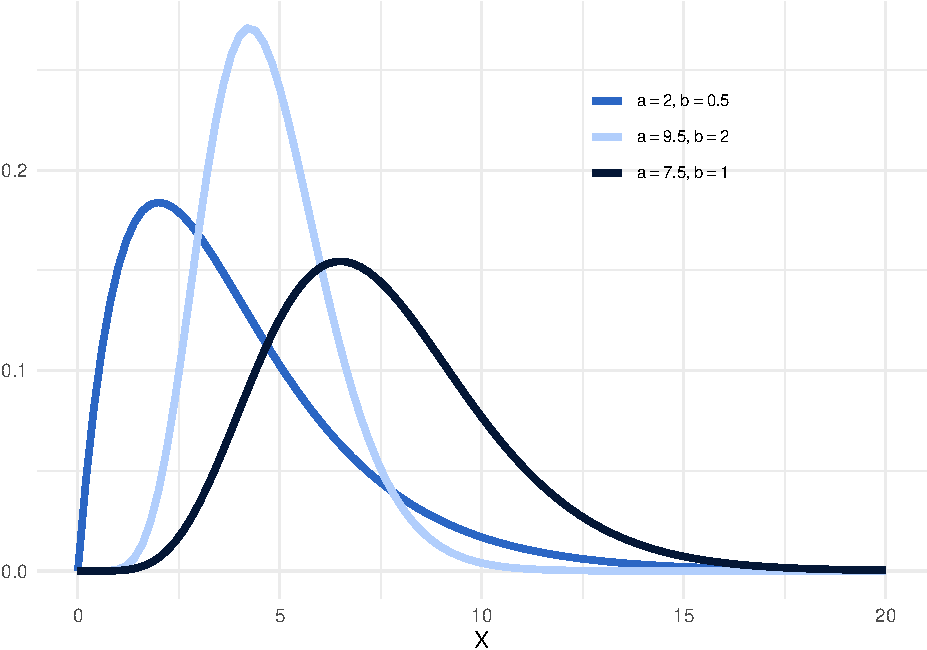
\includegraphics[width=0.8\linewidth]{thesis_files/figure-latex/gamma-1} 

}

\caption{The Gamma(a, b) Distribution}\label{fig:gamma}
\end{figure}
Because the response variable we are working with is strictly positive and often-times right skewed, it's logical to try to model the response as coming from a Gamma distribution. The model is formulated as follows

\[
y_{ij} \sim \text{Gamma}\bigg(\alpha, \frac{\alpha}{\mu_{ij}}\bigg) \qquad \text{where} \qquad \mu_{ij} = \mathbf{x}_{ij}^T\boldsymbol{\beta} + u_j
\]

We are operating under the shape and rate parametrization of a Gamma distribution, and this specific parametrization was chosen so the mean of our response would be the output of the linear component:

\[
E[y_{ij}] = \alpha \bigg(\frac{\alpha}{\mu_{ij}}\bigg)^{-1} = \mu_{ij}
\]

The random intercepts have the same types of prior as in the normal model:

\[
u_j \ | \ \sigma_{u}^2 \sim \mathcal{N}(0, \sigma_{u}^2)
\]

with hyperprior \(\sigma_{u}^2\). We then define priors for the other parameters as

\[
\begin{aligned}
\beta_p &\sim \mathcal{N}(m_p, s_p^2)  \qquad \forall p\in P \\
\alpha &\sim \text{Half-Cauchy}(t_1, r_1^2)\\
\sigma_{u}^2 &\sim \text{Half-Cauchy}(0, r_2^2)
\end{aligned}
\]

where \(m_p, s_p^2, t_1, r_1, r_2\) are real valued numbers. While the Cauchy prior put on the shape parameter \(\alpha\) is still bounded below by zero, we now allow it's mode to be set based on the given data.

Letting \(\boldsymbol{\delta} = (\delta_1, ..., \delta_P)\) and \(\mathbf{u} = (u_1, ..., u_J)\) we can write out the joint posterior distribution as

\[
\begin{aligned}
p(\boldsymbol{\beta}, \mathbf{u}, \sigma_{u}^2, \alpha \ | \ \mathbf{y}) &=\bigg[\prod_{i:y_{i} > 0}p(y_{i} \ | \ \boldsymbol{\beta},\mathbf{u}, \sigma_{u}^2, \alpha)\bigg]\cdot p(\beta_1)\cdot...\cdot p(\beta_P)p(u_1)\cdot ... \cdot p(u_J)p(\sigma_{u}^2)p( \alpha) 
\end{aligned}
\]

Hopefully at this point the repetitiveness of this process and of these formulations has helped to drill home the Bayesian method of model fitting. We've seen it in three different flavors: Logistic regression, Normal regression, and Gamma regression, but all that's really changed at each step has been the link function and the priors and parameters used.

\hypertarget{bayespred}{%
\section{Evaluation of the Bayesian Model: Posterior Predictive Distribution}\label{bayespred}}

In the Frequentist frame the model parameters are treated as fixed but unknown and so once we obtain estimates for them, we simply use those point estimates to make predictions.

\[
\begin{aligned}
\hat{y}^*_{ij} &= \mathbf{x}_{ij}^T\hat{\boldsymbol{\beta}} + \hat{u}_j \\
\hat{p}_{ij} &= \frac{1}{1 + e^{-(\mathbf{x}_{ij}^T\hat{\boldsymbol{\gamma}} + \hat{v}_j)}} \\
\hat{Y}_{j} &= \sum_{i\in n_j}\hat{y}^*_{ij}\cdot \hat{p}_{ij} 
\end{aligned}
\]

But in the Bayesian frame our model parameters are no longer fixed values, but are described by a posterior distribution. Instead of producing predictions that are single values, we construct what are called posterior predictive distributions. In fact it makes sense why we would end up with predictive distributions rather than single values when you consider that there are two main sources of variability that should be taken into account in our predictions:
\begin{enumerate}
\def\labelenumi{\arabic{enumi}.}
\item
  Sampling variability in the data: we never expect our model to be perfectly deterministic, rather the real outcomes should be expected to vary around the model.
\item
  Posterior variability of the model parameters: we shouldn't go through all the trouble of constructing posterior distributions for our parameters to just throw out that information when it comes time to make predictions, rather we incorporate the variability in our posterior distributions into our predictions.
\end{enumerate}
Within the Bayesian frame, these two sources of variability are combined to produce what is called a posterior predictive distribution (Johnson, Ott, \& Dogucu, 2022).

To get a feel for how this works, I'll start by just focusing on constructing a posterior predictive distribution for a new point, \(y_{ij, \ new}\), using each model separately.

\hypertarget{theoretical-version}{%
\subsection{Theoretical version}\label{theoretical-version}}

To really stress the logic of what we're doing, imagine that we haven't collected any data yet and that we only had one parameter \(A\) in our model. In any model we assume that the data for a fixed parameter \(A\) has distribution \(p(y \ | \ A)\). Moreover, before having observed any data, all of our uncertainty about the value of \(A\) is contained by the prior \(p(A)\). We can imagine \(p(y \ | \ A)\) capturing the variability in (1) and \(p(A)\) capturing the variability in (2).

To produce an estimate for the distribution of a new data point \(y_{ij, \ new}\) we simply integrate the product of the previous two terms over \(A\).

\[
\begin{aligned}
\int_A p(y_{ij, \ new} \ | \ A)p(A )dA   = p(y_{ij, \ new} )   \\
\end{aligned}
\]

This is sometimes called the prior predictive distribution for \(y_{ij, \ new}\) as it represents our knowledge about \(y_{ij, \ new}\) before observing any data.

But we can do much better at describing the variability of the model parameters than this. After observing the sample data we update our knowledge. Again we have the same \(p(y_{ij, \ new} \ | \ A)\) which captures the sampling variability in the data, but now the variability of the model parameter is described by the posterior distribution \(p(A \ | \ \mathbf{y})\). Again we get a distribution for \(y_{ij, \ new}\) by integrating over \(A\), except this time we end up with \(p(y_{ij, \ new} \ | \ \mathbf{y})\) which is aptly named the \textbf{posterior predictive distribution}

\[
\begin{aligned}
\int_A p(y_{ij, \ new} \ | \ A, \mathbf{y})p(A \ | \ \mathbf{y})dA &=  \int_A p(y_{ij, \ new} \ | \ A)p(A \ | \ \mathbf{y})dA \qquad y_{ij, \ new} \ \  \text{independent of } \mathbf{y} \\
&= p(y_{ij, \ new} \ | \ \mathbf{y})\
\end{aligned}
\]

Note that the quality of this posterior predictive distribution depends strongly on the quality of our posterior distribution. In other words, this distribution will only accurately capture the structure of new data points, if the underlying posterior distribution correctly captures the structure of the parameters of interest.

As we move on to the expression for each full model, just remember that while the integral looks very complicated, all that we're doing is incorporating both sources of variability and averaging across the possible values of the model parameters. The posterior predictive distribution for a point \(y^*_{ij, \ new}\) using the Normal regression model can be written as:

\[
\begin{aligned}
p(y^*_{ij, \ new} \ | \ \mathbf{y}) &=  \int_{\beta_1}  \dots \int_{\beta_P} \int_{u_1} \dots \int_{u_J} \int_{\sigma_{u}^2} \int_{\sigma_{\varepsilon}^2} \bigg[p(y^*_{ij, \ new} \ | \ \boldsymbol{\beta}, \boldsymbol{u}, \sigma_{u}^2, \sigma_{\varepsilon}^2)p(\boldsymbol{\beta}, \mathbf{u}, \sigma_{u}^2, \sigma_{\varepsilon}^2 \ | \ \mathbf{y})\bigg] \\
& \ \ \ \ \ d\beta_1 ...  d\beta_Pdu_1...du_Jd\sigma_{u}^2d\sigma_{\varepsilon}^2
\end{aligned}
\]

Similarly, for the Gamma model it can be written as

\[
\begin{aligned}
p(y^*_{ij, \ new} \ | \ \mathbf{y}) &=  \int_{\beta_1}  \dots \int_{\beta_P} \int_{u_1} \dots \int_{u_J} \int_{\sigma_{u}^2} \int_{\alpha} \bigg[p(y^*_{ij, \ new} \ | \ \boldsymbol{\beta}, \mathbf{u}, \sigma_{u}^2, \alpha)p(\boldsymbol{\beta}, \mathbf{u}, \sigma_{u}^2, \alpha \ | \ \mathbf{y})\bigg] \\
& \ \ \ \ \ d\beta_1 ...  d\beta_Pdu_1...du_Jd\sigma_{u}^2d\alpha
\end{aligned}
\]

And for the classification model it can be expressed as

\[
\begin{aligned}
p(z_{ij, \ new} \ | \ \mathbf{y}) &=  \int_{\gamma_1}  \dots \int_{\gamma_P} \int_{v_1} \dots \int_{v_J} \int_{\sigma_{v}^2}  \bigg[p(z_{ij, \ new} \ | \ \boldsymbol{\gamma}, \mathbf{v}, \sigma_{v}^2)p(\boldsymbol{\gamma}, \mathbf{v}, \sigma_{v}^2 \ | \ \mathbf{y})\bigg] \\
& \ \ \ \ \ d\gamma_1 ...  d\gamma_Pdv_1...dv_Jd\sigma_{v}^2
\end{aligned}
\]

The distributions \(p(y^*_{ij, \ new} \ | \ \mathbf{y})\) and \(p(z_{ij, \ new}\ | \ \mathbf{y})\) not only capture where we think each prediction might lie, but also how we would expect it to vary. Often in predictive modeling we're interested in quantifying the uncertainty in our model estimates, and in the Bayesian framework these are baked right into the predictions themselves.

While the theory behind constructing these posterior predictive is pretty intuitive, it's clear that even in the case of a fairly simple model, the actual computations are rather unwieldy. Again, we are saved by the fact that in practice the posterior is too complex to algebraically solve for, so we're already functioning in a setting where we use MCMC to simulate draws from the approximate posterior.

\hypertarget{mcmc-version}{%
\subsection{MCMC version}\label{mcmc-version}}

First I will describe how the posterior predictive distribution is derived from the MCMC draws, and then I will explain how it approximates the exact calculation above.

To generate a posterior predictive distribution for a new data point \(y_{ij,\ new}\) using the normal regression model we simulate a prediction from the model for each parameter set of the MCMC output.

\[
\begin{bmatrix}
y_{ij, \ new}^{(1)} \sim \mathcal{N}\Big( \mathbf{x}_{ij, \ new}^T \boldsymbol{\beta}^{(1)} + u_j^{(1)}, (\sigma_{\varepsilon}^2)^{(1)}\Big) \\
\\
\vdots \\
\\
y_{ij, \ new}^{(2000)} \sim \mathcal{N}\Big(\mathbf{x}_{ij, \ new}^T \boldsymbol{\beta}^{(2000)} + u_j^{(2000)}, (\sigma_{\varepsilon}^2)^{(2000)}\Big)
\end{bmatrix}
\]

The result is a set \(\Big\{y_{ij , \ new}^{(1)}, y_{ij, \ new}^{(2)}, ..., y_{ij, \ new}^{(2000)}\Big\}\) which approximates the posterior predictive distribution.

For the Gamma model we do the same thing but using the appropriate distribution

\[
\begin{bmatrix}
y_{ij, \ new}^{(1)} \sim \text{Gamma}\Bigg(\alpha^{(1)}, \frac{\alpha^{(1)}}{ \mathbf{x}_{ij, \ new}^T\cdot \boldsymbol{\beta}^{(1)} + u_j^{(1)}}\Bigg) \\
\\
\vdots \\
\\
y_{ij, \ new}^{(2000)} \sim \text{Gamma}\Bigg(\alpha^{(2000)}, \frac{\alpha^{(2000)}}{ \mathbf{x}_{ij, \ new}^T\cdot \boldsymbol{\beta}^{(2000)} + u_j^{(2000)}}\Bigg)
\end{bmatrix}
\]

And we do the same thing for the classification model

\[
\begin{bmatrix}
z_{ij, \ new}^{(1)} \sim \text{Bernoulli}\Bigg(\frac{1}{1 + e^{-\big(\mathbf{x}_{ij}^T\boldsymbol{\gamma}^{(1)} + v_j^{(1)}\big)}}\Bigg) \\
\\ \vdots \\ \\
z_{ij, \ new}^{(2000)} \sim \text{Bernoulli}\Bigg(\frac{1}{1 + e^{-\big(\mathbf{x}_{ij}^T\boldsymbol{\gamma}^{(2000)} + v_j^{(2000)}\big)}}\Bigg)
\end{bmatrix}
\]

While it may not be immediately clear, these processes are really just mimicking what the massive integrals above were computing exactly. By simulating realizations of the distribution behind each model, we are again capturing the sampling variability in the data, and by doing so across all of our MCMC parameter draws, the uncertainty about the model parameters is being incorporated as well.

\hypertarget{combining-the-model-predictions}{%
\subsection{Combining the Model Predictions}\label{combining-the-model-predictions}}

Now that we have two sets which represent approximate the posterior predictive distribution for unit \(i\) in group \(j\) for each respective model, we have to think about how we combine them. After all, our final model prediction is the product of these two models, So we certainly need a posterior predictive distribution of \(y_{ij, \ new} = y_{ij, \ new}^*p_{ij, \ new}\), but it's unclear how we should combine the predictive distributions from the individual models to get here. In the Frequentist version where our predictions are single point values, this poses no problem at all, but now that our predictions are themselves distributions, it's a little less clear how to proceed. We might just match MCMC iteration \(k\) from each model together, but what makes this matching more correct than shuffling the iterations and then matching them up?

One solution to this conundrum of combining the distributions is to simply build the models simultaneously. In practice this relies on a few tricks and definitely increases the complexity when actually writing code for it, but it can be done and it does allow us to avoid this problem. That being said, as the two models grow to be more complicated, this process of building them simultaneously grows much more difficult and so it isn't a very robust solution to the problem. In the next section we walk through a nice theoretical finding that offers a solution to this problem.

\hypertarget{sepsim}{%
\section{Simultaneous v.s Separate}\label{sepsim}}

\hypertarget{simultaneous-model-build}{%
\subsection{Simultaneous Model Build}\label{simultaneous-model-build}}

As we just mentioned, to get around our problem of how we combine the MCMC iterations for the models built separately, we could fit the models simultaneously. The one major assumption that we will have here is that there is no dependence in the priors \textbf{between} models. While there are certainly cases where this doesn't hold, trying to incorporate these dependencies into the model incorporate a lot more complexity without much performance gain\footnote{Pfeffermann, Terryn, \& Moura (2008)}.

Finally, this result holds regardless of the particular models that we use, but for the sake of simplicity we'll use a logistic regression model with no random effects and a Normal linear regression model with no random effects. As mentioned above, we have to get a bit crafty when building the models simultaneously and the way we do this is as follows. First we fit the logistic regression model as we normally would:

\[
z_{ij} \sim \text{Bernoulli}\Bigg(\frac{1}{1 + e^{-\mu_{ij}}}\Bigg) \qquad \text{where} \qquad \mu_{ij} =\mathbf{x}_{ij}^T\boldsymbol{\gamma} + v_j
\]

But then the two part process gets folded into the way that we set up the Normal linear regression model:

\[
y_{ij} \sim \mathcal{N}\bigg(z_{ij}\cdot m_{ij} \ , \ \Big[z_{ij}\cdot\tau_1 + (1 - z_{ij})\tau_2\Big]\bigg) \qquad \text{where} \qquad m_{ij} =\mathbf{x}_{ij}^T\boldsymbol{\beta} + u_j
\]

Here \(\tau_1\) represents the variance of \(y_{ij}\) when \(z_{ij} = 1\) and thus can be estimated, but \(\tau_2\) is the variance of \(y_{ij}\) when \(z_{ij} = 0\) and so there's no practical way for it to be estimated by the MCMC algorithm. The solution is to just set \(\tau_2\) as some small fixed number (i.e \(0.001\)) and approximate the posterior for all the other parameters.

With all of that in mind, in this setting our posterior for both models would be:

\[
\begin{aligned}
p(\boldsymbol{\beta}, \boldsymbol{\gamma}, \mathbf{u}, \mathbf{v}, \sigma_u^2, \sigma_v^2, \tau_1\ | \ \mathbf{y}) &\propto p(\mathbf{y} \ | \boldsymbol{\beta}, \boldsymbol{\gamma}, \mathbf{u}, \mathbf{v}, \sigma_u^2, \sigma_v^2, \tau_1)p(\boldsymbol{\beta}, \boldsymbol{\gamma}, \mathbf{u}, \mathbf{v}, \sigma_u^2, \sigma_v^2, \tau_1) 
\end{aligned}
\]

We can expand this by writing out the likelihood more fully based on whether \(y\) is zero or not:

\[
\begin{aligned}
p(\boldsymbol{\beta}, \boldsymbol{\gamma}, \mathbf{u}, \mathbf{v}, \sigma_u^2, \sigma_v^2, \tau_1 \ | \ \mathbf{y}) & \propto \bigg[\prod_{i:y_i = 0}(1-p_i)\prod_{i:y_i > 0}(p_i)p(y_i \ | \ \boldsymbol{\beta}, \mathbf{u}, \sigma_u^2, \tau_1)\bigg]\cdot  p(\boldsymbol{\beta}, \boldsymbol{\gamma}, \mathbf{u}, \mathbf{v}, \sigma_u^2, \sigma_v^2, \tau_1)\\
\end{aligned}
\]

While it wasn't too difficult to write this out up to a proportionality constant, in practice it can be very difficult to figure out how to combine the two models in such a way that the MCMC algorithm still converges once you start using models that are more complicated than these ones.

But, there's important insight still to be found here. Let's group these terms based on the parameters that they use. In particular we'll group by which individual model the parameter belongs to:

\[
\begin{aligned}
&= \Bigg[\Big(\prod_{i:y_i = 0}(1- p_i)\prod_{i: y_i > 0}p_i\Big)p(\boldsymbol{\gamma}, \mathbf{v}, \sigma_v^2)\Bigg]\Bigg[\Big(\prod_{i:y_i > 0}p(y_i \ | \ \boldsymbol{\beta}, \mathbf{u}, \sigma_u^2, \tau_1)\Big)p(\boldsymbol{\beta},\mathbf{u}, \sigma_u^2, \tau_1)\Bigg]
\end{aligned}
\]

Again, we are able to split the joint prior in this way because we are assuming that there is no dependence in the priors \textbf{between} models.

But now, if we look at this closely we can see that what we really have here is a full separation into the posteriors for the individual models for \(p\) and \(y^*\) as seen in our derivation in the previous section. This means that we can write:

\[
\begin{aligned}
p(\boldsymbol{\beta}, \boldsymbol{\gamma}, \mathbf{u}, \mathbf{v}, \sigma_u^2, \sigma_v^2, \tau_1\ | \ \mathbf{y})  &\propto p(\boldsymbol{\beta}, \mathbf{u}, \sigma_u^2, \tau_1 \ | \ \mathbf{y})p(\boldsymbol{\gamma}, \mathbf{v}, \sigma_v^2 \ | \ \mathbf{y}) \\
  &= C\bigg[p(\boldsymbol{\beta}, \mathbf{u}, \sigma_u^2, \tau_1 \ | \ \mathbf{y})p(\boldsymbol{\gamma}, \mathbf{v}, \sigma_v^2 \ | \ \mathbf{y})\bigg]
\end{aligned}
\]

Finally, since these are all proper probability distributions we know that they should all integrate to 1 when integrated across all of their parameters. If we integrate both sides over all of the parameters from both models, its clear that the LHS would be one, and once we recall that there is no parameter dependence \textbf{between} the models, it is clear that the RHS does as well. And so we are left with the conclusion that \(C = 1\) and thus that

\[
p(\boldsymbol{\beta}, \boldsymbol{\gamma}, \mathbf{u}, \mathbf{v}, \sigma_u^2, \sigma_v^2, \tau_1\ | \ \mathbf{y})  = p(\boldsymbol{\beta}, \mathbf{u}, \sigma_u^2, \tau_1 \ | \ \mathbf{y})p(\boldsymbol{\gamma}, \mathbf{v}, \sigma_v^2 \ | \ \mathbf{y}) 
\]

So the full posterior for the model built simultaneously is equal to the product of the posteriors for each model built separately. The major upshot here is that we can fit the models separately, and then combine the results at the end to get our posterior predictive distributions. In other words \emph{as long as we don't build in any correlations between the parameters in the two models, then we can build each model as complex as we might desire without having to worry about how we will eventually build the two models together. As we learned above, we can simply build them separately and combine the results at the end.}. This is a really nice theoretical finding as it alleviates the need to figure out how to build the models simultaneously and encourages us to have freedom in how we build each individual model.

\hypertarget{practical-backing}{%
\subsection{Practical Backing}\label{practical-backing}}

To test our theoretical work above, we fit simpler versions of the two models with no random effects. And indeed, when we fit the models simultaneously and also fit them separately making use of MCMC to simulate samples from their approximate posteriors, we find that they are practically identical.
\begin{center}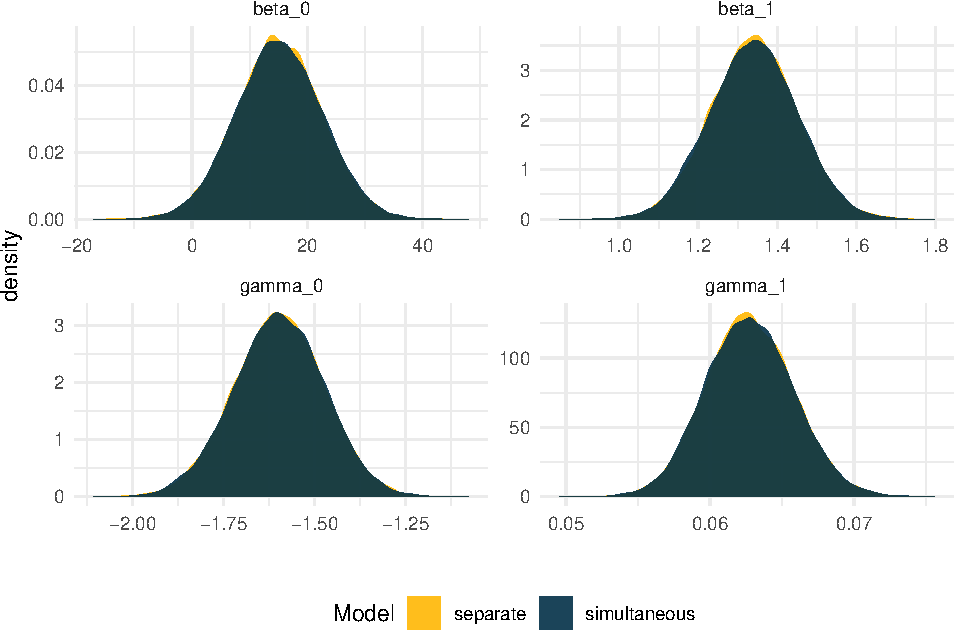
\includegraphics[width=0.8\linewidth]{thesis_files/figure-latex/unnamed-chunk-3-1} \end{center}

\hypertarget{wrapone}{%
\section{Posterior Predictive Distribution Finalized}\label{wrapone}}

Now that we know that we can fit the models separately and then combine them at the end, we are finally ready to describe how final predictions are made.

Since we are interested in a making predictions for the average response in group \(j\) we obtain a set that approximates the posterior predictive distribution for each unit \(i\) in group \(j\). For example, if we fix \(j\) and let \(n_j = 5\) we would have 5 sets:

\[
\begin{aligned}
&\Big\{y_{1j , \ new}^{(1)}, \ y_{1j, \ new}^{(2)}, ..., \ y_{1j, \ new}^{(2000)}\Big\} \\
&\Big\{y_{2j , \ new}^{(1)}, \ y_{2j, \ new}^{(2)}, ...,  \ y_{2j, \ new}^{(2000)}\Big\} \\
& \qquad \qquad \qquad \ \   \vdots \\
&\Big\{y_{5j , \ new}^{(1)}, \ y_{5j, \ new}^{(2)}, ..., \ y_{5j, \ new}^{(2000)}\Big\}
\end{aligned}
\]

To get the posterior predictive distribution for \(\bar{y}_{j, \ new}\) we take averages across units in group \(j\) by indices of the MCMC draws. In other words we take the average of \(\Big\{y_{1j, \ new}^{(k)}, y_{2j, \ new}^{(k)}, ... , y_{5j, \ new}^{(k)}\Big\}\) for each MCMC draw \(k\). In full we end up with the set:

\[
\begin{bmatrix}
\frac{1}{n_j} \sum_{i = 1}^{n_j}\hat{y}_{ij, \ new}^{(1)} \\
\frac{1}{n_j} \sum_{i = 1}^{n_j}\hat{y}_{ij, \ new}^{(2)} \\
\vdots \\
\frac{1}{n_j} \sum_{i = 1}^{n_j}\hat{y}_{ij, \ new}^{(2000)}
\end{bmatrix} \qquad = \qquad 
\begin{bmatrix}
\hat{Y}_{j, \ new}^{(1)} \\
\hat{Y}_{j, \ new}^{(2)} \\
\vdots \\
\hat{Y}_{j, \ new}^{(2000)}
\end{bmatrix}
\]

Which is an approximation of the posterior predictive distribution for the mean of the response in group \(j\).

\hypertarget{wraptwo}{%
\section{Prediction Intervals}\label{wraptwo}}

In statistical modeling, another piece of information that we're often interested is a measure of our uncertainty in our predicted values. Often times these are referred to broadly as prediction intervals, and whereas the confidence intervals and credible intervals that we described in Chapter \ref{bayes-freq} provide uncertainty bounds for parameter estimates, these prediction intervals provide uncertainty bounds for a future observation or data point.

Immediately, we can see how straightforward it is to acquire these in the Bayesian setting. Because our predictions are not simply point estimates, but are predictions themselves, these prediction intervals are baked right into the prediction process.

Unfortunately it is far less straightforward in the Frequentist setting. While prediction intervals are straightforward to generate for singular regression models, things get a lot more complicated with a two part model like ours. The reality is that we spent a good amount of time trying to construct a bootstrap procedure to generate these prediction intervals and beyond being very computationally intensive, we also couldn't find one that actually worked correctly. While this was certainly frustrating, the struggle to try to develop a process for generating these prediction intervals for the Frequentist models, really highlighted how nice it is that you get them for free in the Bayesian model.

\hypertarget{a-note-of-caution}{%
\subsubsection{A note of caution}\label{a-note-of-caution}}

While it might be tempting to gleefully pronounce Bayesian models to be better than Frequentist simply for the ease of access to prediction intervals, the important caveat is that these prediction intervals will only be correct when the Bayesian model is correct. What I mean by that is that if our Bayesian model badly fits the data, then we still get uncertainty estiamtes for free, but a 95\% prediction interval will likely not get 95\% coverage, thus indicating that the intervals themselves are also incorrect.

\hypertarget{sim-study}{%
\chapter{Simulation Study}\label{sim-study}}

We now introduce and the set up for the simulation study that will be the main avenue through which we evaluate the various models.

\hypertarget{aims}{%
\section{Aims}\label{aims}}

The first aim for this simulation study is to understand when we might benefit from using a Bayesian model.

In order to try to answer this question of \emph{when} we will be turning a few dials. Because we are functioning in a setting with grouped data with moderately small sample sizes we will vary the data along two axes
\begin{itemize}
\tightlist
\item
  Number of groups
\item
  Number of observations per group
\end{itemize}
The second aim is to get a sense for the role that the prior plays in a Bayesian analysis. To do so we will vary the quality of the priors put on the model parameters. The two levels will be
\begin{itemize}
\tightlist
\item
  Uninformative
\item
  Informative
\end{itemize}
The idea to vary the quality of the priors comes out of the idea that while the likelihood does dominate the prior in large sample size settings, the prior plays a much larger role in smaller sample settings and thus we might expect a lot more regularization and model convergence in the Bayesian models when more information is added through the priors.

\hypertarget{data-and-dials}{%
\section{Data and Dials}\label{data-and-dials}}

\hypertarget{estimands}{%
\subsection{Estimands}\label{estimands}}

The primary estimand for this simulation study will be \(Y_j\): the mean of our response variable in domain \(j\). In order to stay consistent across all models and simulation runs, we only made predictions on group \(1\).

\hypertarget{data-generating-process}{%
\subsection{Data Generating Process}\label{data-generating-process}}

Our population data for the simulation was generated by the following process that takes as inputs the number of domains (\(J\)) and the number of total observations (\(N\)). The number of observations per group is thus (\(n = N/J\)). The population was generated using \(N = 50\cdot 500\) and \(J = 50\), to give us 500 observations per group.

The DGP is defined as follows

\[
\begin{aligned}
z_{ij} &\sim \text{Bernoulli}(p_{ij}) \ \ \ \ \text{where} \ \ \ \ p_{ij} = \frac{\text{exp}\big(1.5 + X_{ij} + v_j\big)}{1 + \text{exp}\big(1.5 + X_{ij} + v_j\big)} \\
y^*_{ij} &\sim \text{Gamma}(3, \  1/b_{ij}) \ \ \ \ \text{where} \ \ \ \ b_{ij} = 10 + X_{ij} + u_{j} \\
y_{ij} &=z_{ij}\cdot y^*_{ij}
\end{aligned}
\]

Where \(X_{ij} \overset{\text{iid}}{\sim} \mathcal{N}(0, 1)\), \(v_j \overset{\text{iid}}{\sim} \mathcal{N}(0, 1)\) and \(u_{ij} \overset{\text{iid}}{\sim} \mathcal{N}(0, 1)\)

This data generating process checks all of our boxes as it produces zero-inflated data with a grouped structure and a moderate relationship between the response \(Y\) and a covariate \(X\). For example if we examine the generated population data we see the following.

The response variable is indeed zero inflated with a strictly positive and continuous non-zero portion.
\begin{figure}

{\centering 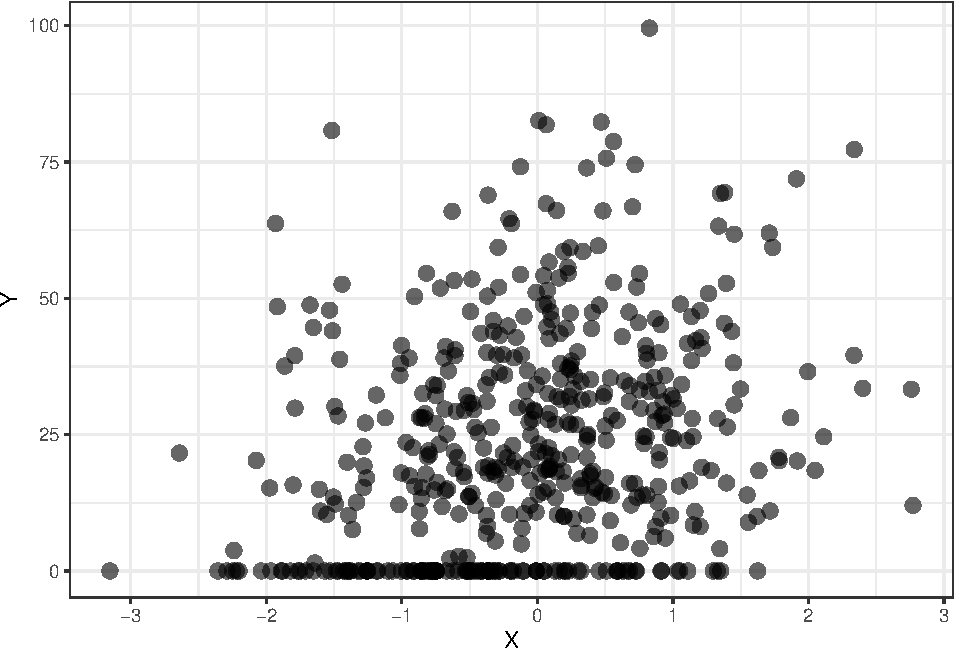
\includegraphics[width=0.8\linewidth]{thesis_files/figure-latex/unnamed-chunk-5-1} 

}

\caption{The distribution of the response variable in the population that we generated for our simulation.}\label{fig:unnamed-chunk-5}
\end{figure}
If we examine the correlation between \(X\) and \(Y\) we get 0.305, for the entire data set. And indeed when we examine the plot of \(Y\) against \(X\) we do see a relationship. Here we just plot points from a single group so as not to overclutter the plot.
\begin{figure}

{\centering 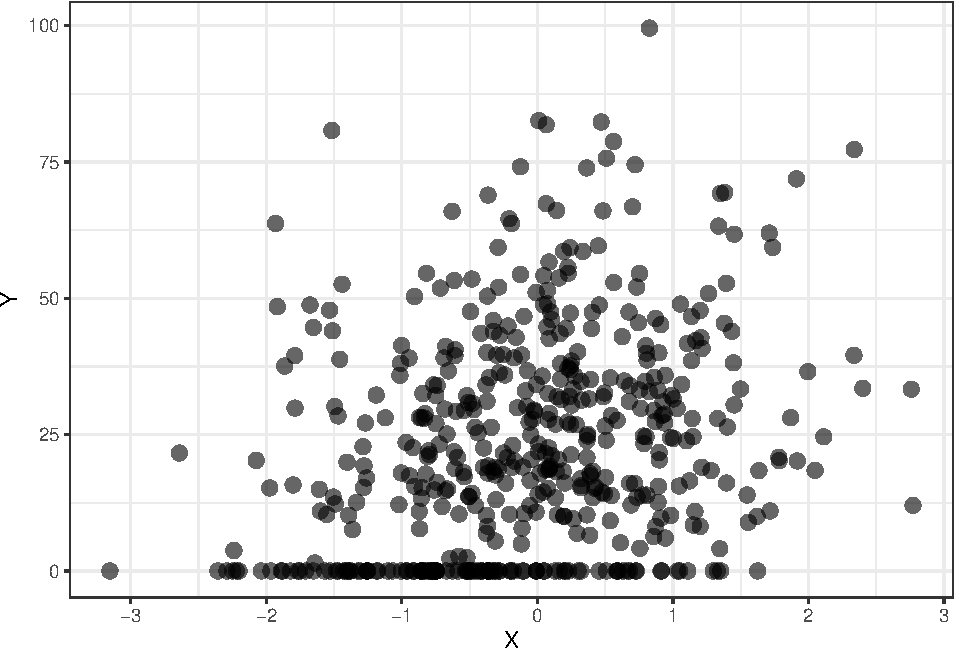
\includegraphics[width=0.8\linewidth]{thesis_files/figure-latex/unnamed-chunk-6-1} 

}

\caption{Scatterplot of the main covariate against the response variable in Group 1 of our generated population data.}\label{fig:unnamed-chunk-6}
\end{figure}
\hypertarget{dials}{%
\subsection{Dials}\label{dials}}

The exact levels of the dials for number of groups and number of observations per group will be
\begin{itemize}
\tightlist
\item
  n = \(\{15, 30, 50\}\)
\item
  J = \(\{5, 10, 25, 50\}\)
\end{itemize}
We ran a simulation for each combination of those levels, for a total of 12 runs, to get a full sense of how the models perform across each of these measures of how ``small'' the data is. In order to generate data sets for these settings we first sampled \(J\) groups from the population, and then within those groups we sampled \(n\) observations. Importantly, because we were always predicting on group 1, we always forced that group into each simulation iteration. For each of the 12 individual settings we ran 400 total iterations of the simulation.

Next, within each \((n,\ J)\) combination we built the Bayesian models with two types of priors: Non-Informative and Informative. Note that across our models we have a variety of parameters that require priors.
\begin{itemize}
\item
  For the Normal regression model we have the the fixed effects coefficients \((\boldsymbol{\beta})\), the variance parameter for the random intercepts \((\sigma_u^2)\), and the variance parameter for the observation level model error \((\sigma_{\varepsilon}^2)\).
\item
  For the Gamma regression model we once again have the fixed effects coefficients \((\boldsymbol{\beta})\), and the variance parameter for the random intercepts \((\sigma_u^2)\), but this time we also have the shape parameter \((\alpha)\).
\item
  For the Logistic regression model we have new fixed effects coefficients \((\boldsymbol{\gamma})\) and the variance parameter for the random intercepts \((\sigma_v^2)\).
\end{itemize}
Note that across all models the random effects are assumed to be \(\mathcal{N}(0, \tau^2)\) distributed and thus can be thought of as universally having a normal prior with a variance hyperparameter. While the distributions chosen for these priors were introduced in the methods section, we will now choose real valued numbers used to center and scale those priors.

These parameters that require priors can be placed into 3 main groups: fixed effects, variance, and shape. We simplified the process of assigning the levels of priors by not varying the priors within these groups within each bracket of quality.

\hypertarget{non-informative}{%
\subsubsection{Non-Informative}\label{non-informative}}

In order to include no prior knowledge in your analysis, a flat prior can be used: \(p(\theta) \propto 1\). Recall that the posterior can be factored into a normalized product of the likelihood and the prior. Thus, to use a flat, non-informative, prior is to ``let the data speak for itself'' and utilize only the likelihood function in estimating the posterior. That being said prior distributions should still not cover parameter values that are impossible, and thus the flat priors will have supports that are restricted to the range of possible values that the parameter could take on. For the fixed effects parameters a support of \((-100, 100)\) was used and for the variance and shape parameters \((0, 100)\) was used.
\begin{center}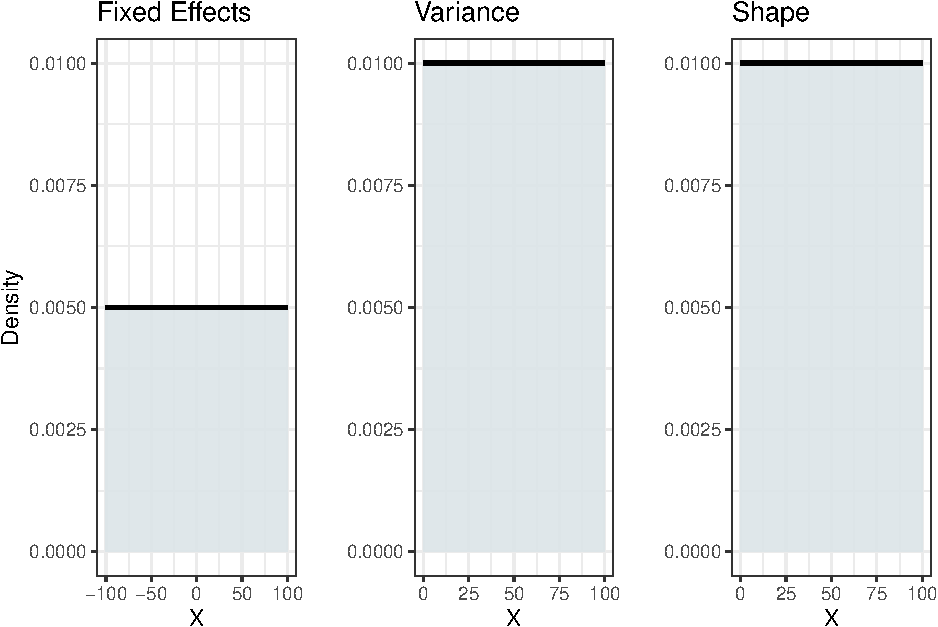
\includegraphics[width=0.8\linewidth]{thesis_files/figure-latex/unnamed-chunk-8-1} \end{center}

\hypertarget{info}{%
\subsubsection{Informative}\label{info}}

Next, the goal with our informative priors was add more information by choosing to center and scale the prior distributions with the observed data in mind. Naturally, since we know the exact process that generated the data it might be tempting to center the priors exactly on the correct parameter values, but to do so would certainly be both unfair and unrealistic. Instead exploratory data analysis was utilized to make the decisions.

An examination of a scatterplot of the response and covariate leads us to believe that the fixed effects coefficients for the models fitting the non-zero portion of the response are small \emph{positive} numbers between the range of 0 to 10 and thus the prior \(\mathcal{N}(5, 3^2)\) was used.
\begin{center}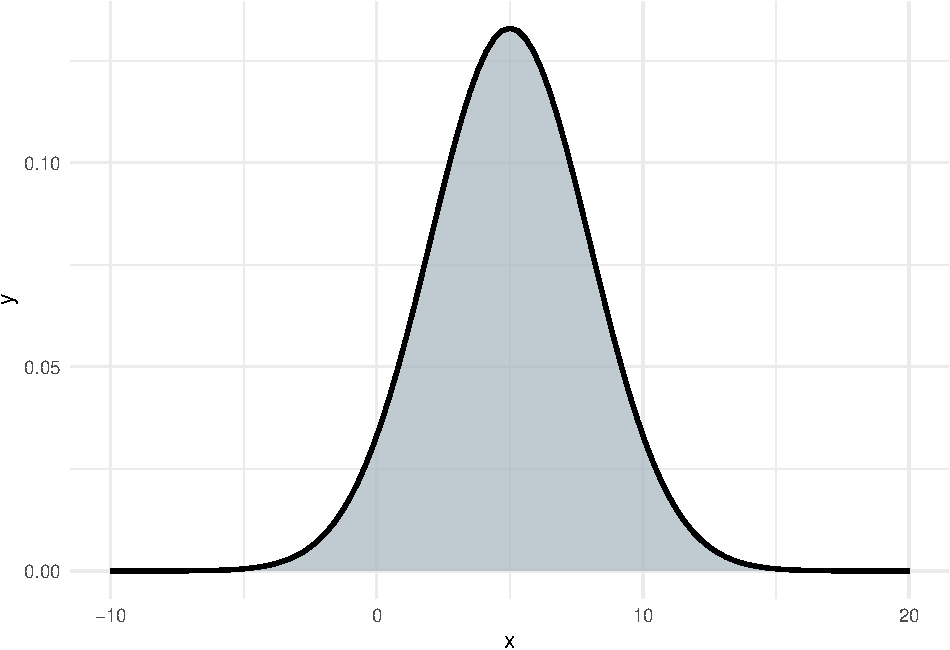
\includegraphics[width=0.8\linewidth]{thesis_files/figure-latex/unnamed-chunk-9-1} \end{center}

On the other hand, we tweaked the scale of this prior for the logistic regression model since the response being modeled is on a different scale. At this point we don't have much of an idea of how the chance of being non-zero changes as the covariate changes, so we use a \(\mathcal{N}(1,1)\) prior for the fixed effects coefficients in the logistic regression model (this may seem like a tight distribution, but in the context of logistic regression slope coefficients it's really quite wide).

Next, following the advice of \footnote{Gelman (2006)} the scale parameter of \(2.5\) was used to parametrize the Cauchy prior put on all variance parameters. In full the \(\text{Half-Cauchy}(0, 2.5)\) prior was utilized.
\begin{center}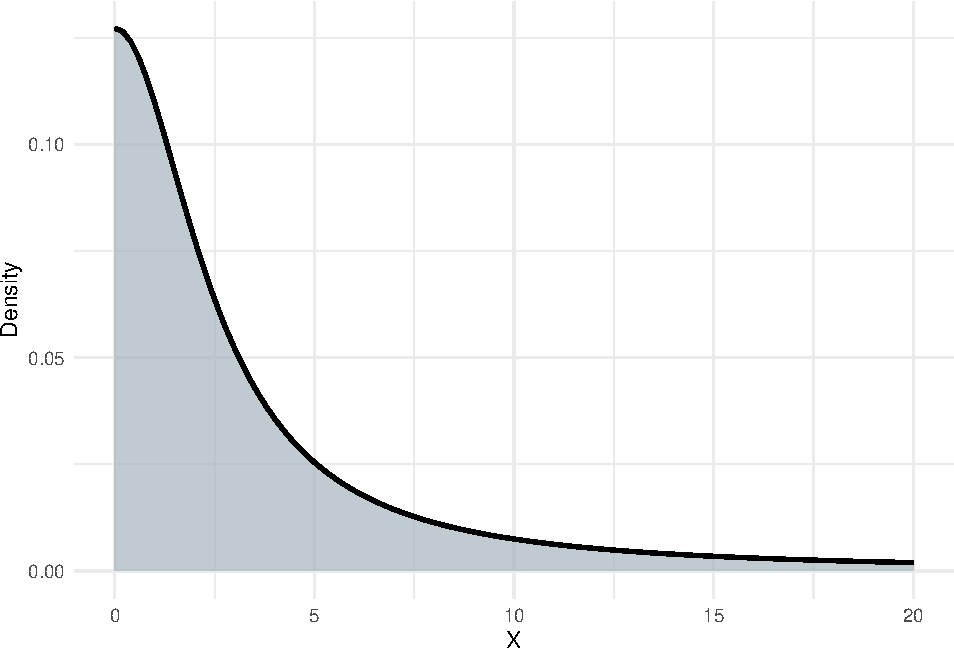
\includegraphics[width=0.8\linewidth]{thesis_files/figure-latex/unnamed-chunk-10-1} \end{center}

Finally, since the non-zero portion of the response variable has a mean of 31.12, we can use the following ``back of the napkin'' calculation to get an idea for what the shape parameter should be centered on. Recall that a \(\text{Gamma}(\alpha, \beta)\) distribution has mean \(\alpha / \beta\) and variance \(\alpha / \beta^2\).

\[
\bar{y} = 31.4 \approx \frac{\alpha}{\beta}\qquad \text{and} \qquad s^2 = 338.8 \approx \frac{\alpha}{\beta^2}
\]

But some algebra tells us then that

\[
\frac{\bar{y}}{s^2} = 0.09 \approx \frac{\alpha / \beta}{\alpha / \beta^2} = \beta 
\]

but now plugging in our approximate value for \(\beta\) gives us

\[
\frac{\alpha}{0.09} \approx 31.4 \implies \alpha \approx 2.8
\]

And so we might guess that the shape parameter is around 3. Obviously this calculation will vary quite a bit depending on the sample that we generate, so we use the scale parameter of 5 to emphasize our uncertainty in that estimate. Thus the complete prior used was \(\text{Half-Cauchy}(3, 5)\).
\begin{center}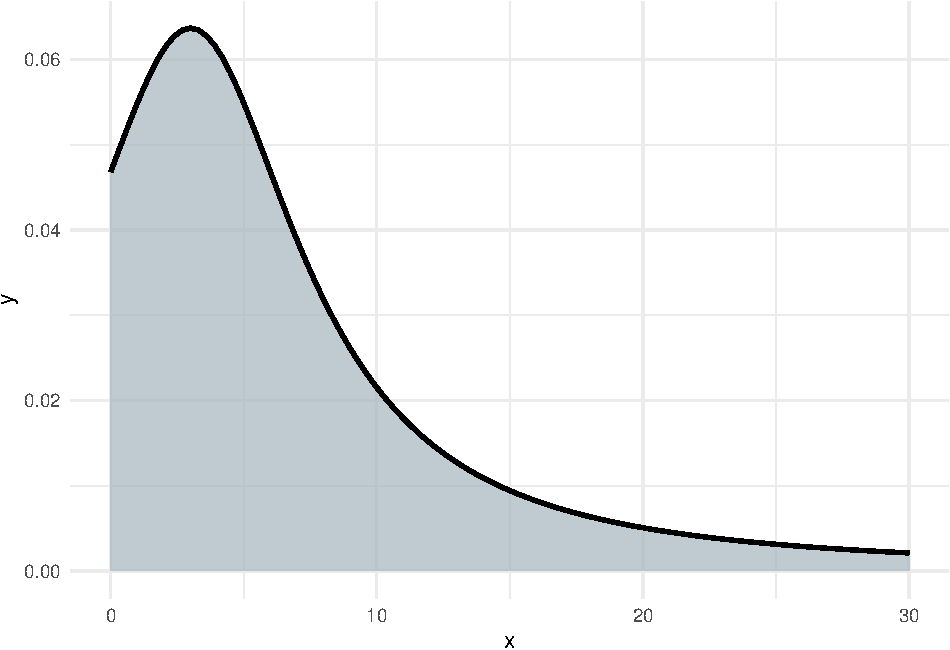
\includegraphics[width=0.8\linewidth]{thesis_files/figure-latex/unnamed-chunk-11-1} \end{center}

\hypertarget{methods}{%
\section{Methods}\label{methods}}

There will be 3 different models run throughout the simulation.
\begin{itemize}
\tightlist
\item
  Frequentist two-part:
  \begin{itemize}
  \tightlist
  \item
    Linear Random Effects Model (\texttt{lme4::lmer})
  \item
    Logistic regression Random Effects Model (\texttt{lme4::glmer})
  \end{itemize}
\item
  Bayesian two-part \#1
  \begin{itemize}
  \tightlist
  \item
    Bayesian Linear Random Effects Model (\texttt{rstanarm::stan\_lmer})
  \item
    Bayesian Generalized Linear Random Effects Model (Binomial) (\texttt{rstanarm::stan\_glmer})
  \end{itemize}
\item
  Bayesian two-part \#2
  \begin{itemize}
  \tightlist
  \item
    Bayesian Generalized Linear Random Effects Model (Gamma) (\texttt{rstanarm::stan\_glmer})
  \item
    Bayesian Generalized Linear Random Effects Model (Binomial) (\texttt{rstanarm::stan\_glmer})
  \end{itemize}
\end{itemize}
\hypertarget{metrics}{%
\section{Performance metrics}\label{metrics}}

Importantly, due to the fact that our data has a clustered structure, we chose to evaluate all of our models on a single group. Thus all of the following performance metrics were computed for the same individual group (group 1) which had a true mean value of \(Y_1 = 23.7\)

The most broadly used and expected performance metric of an estimator is the Mean Squared Error (MSE). We use the Root Mean Squared Error (RMSE) which is computed as follows:

\[
\text{RMSE}_j  = \sqrt{\frac{1}{S}\sum_{s = 1}^{S}\bigg(\hat{\mu}^y_{j, s} - Y_{j}\bigg)^2}
\]

Where \(S\) is the total number of simulation reps, \(\hat{\mu}_{j, s}\) is the estimated mean of the response variable \(y\) in domain \(j\) for simulation rep \(s\), and \(\mu_{j, s}\) is the true mean of the response variable \(y\) in domain \(j\) for simulation rep \(s\).

Next we will be examining the Empirical Bias of each model:

\[
\text{Empirical Bias}_j = E[\hat{\mu}_j] - Y_{j} \qquad \text{where} \qquad E[\hat{\mu}_j] = \frac{1}{S}\sum_{s = 1}^S\hat{\mu}_{j, s}
\]

As well as the Empirical Variance of each model:

\[
\text{Empirical Var}_j  = \frac{1}{(S-1)}\sum_{s = 1}^S\Big(\hat{\mu}_{j,s} - E[\hat{\mu}_j]\Big)
\]

We will look at Predictive Interval (PI) coverage at a 95\% confidence level for the Bayesian Models:

\[
\text{Coverage}_j = \frac{1}{S}\sum_{s = 1}^S \mathbb{I}(Y_{j} \in \text{PI}(\hat{\mu}_{j, s}))
\]

And finally we will look at the total number of model failures.
\begin{itemize}
\tightlist
\item
  For the Frequentist models, a model failure was registered whenever one of the ``Model failed to converge'' warnings from \texttt{lme4}, although even in small sample sizes our data was robust enough that we essentially saw zero model failures.
\item
  For the Bayesian models, a model failure was registered whenever the MCMC algorithm failed one or more of the diagnostics that indicate that the algorithm has converged and is stable. The Stan programming language is robust enough that you should never trust the results when one of these warnings are administered, and so while potentially overly harsh in some cases, we chose to count any convergence warning as a model failure.
\end{itemize}
Importantly, one solution to combating MCMC convergence issues is to bump up the number of iterations that the algorithm progresses through. That being said, this is not a sure fire solution, and always comes at the cost of longer computation time. The default number of iterations is 2000 and is considered a reasonable number of iterations for most models. Because the models we are fitting are fairly complex, ran a few tests to guage how many iterations we should use in order to try to minimize model failures while keeping model run-times reasonable. We saw good improvements up to 5000 iterations and then diminishing returns afterwards, so we used 5000 iterations for all of our Bayesian models.

\hypertarget{res-sec}{%
\chapter{Results}\label{res-sec}}

We now present the results from the simulation study. Each section compares each model with regards to a specific performance metric as laid out in Section \ref{metrics}. Across all of these sections we will label simulation settings like \(n = \cdot\) - \(J = \cdot\). For example if we have \((n = 15, J = 10 )\) it's important to remember that this means that the data sets used in that simulation setting had 10 groups each with 15 observations, and thus the models were trained on \(n\times J = 150\) data points.

Additionally, since the logistic regression component remained the same across all of the Bayesian models, we will use the following syntax when refering to the bayesian models.
\begin{itemize}
\tightlist
\item
  {[}Type of priors, distribution used to model the non-zero response{]}
\end{itemize}
For example, {[}Flat Priors, Normal{]} refers to the Bayesian model that used flat priors and modeled the non-zero response using the Normal distribution.

\hypertarget{expectations}{%
\section{Expectations}\label{expectations}}

Before diving into the actual results, we'll first give a brief overview of what we were expecting to see.

One of the main expectations we had was that we'd see improvements of some kind when using Bayesian models with informative priors compared to Bayesian models with flat priors. At the very least, we hoped to see that the informative priors would assist in reducing the rate at which Bayesian models failed to converge in small sample size settings.

Secondly, we expected to see slightly higher bias in the Bayesian models as compared to the Frequentist models. The reason for this is that our data was generated in a Frequentist way. The parameters were set as fixed constants and not as random variables as a Bayesian conceptualizes them to be. Therefore the Bayesian models should be slightly misspecified and thus should pick up some bias.

With these expectations in mind, we'll now move to the actual results.

\hypertarget{model-failures}{%
\section{Model Failures}\label{model-failures}}

Before we get into the bulk of the performance metrics, we will first examine how often each model failed in each setting across the 400 simulation reps that we ran.

This grid is organized so that the setting with the smallest sample sizes and smallest number of groups is in the top right hand corner. As we move left and down across the grid we move into settings with larger sample sizes and larger number of groups. We can understand the ``size'' of our data in each simulation setting to be a combination of both of these dials and thus we have the following structure.

\[
\begin{bmatrix}
 &  & \text{smallest} \\
 & & & \\
 & \swarrow &  \\
 & & & \\
\text{largest} & & 
\end{bmatrix}
\]

Importantly we omit the Frequentist model in the following plot because it registered no model failures across the entire simulation. The model failure-rate results are as follows:
\begin{figure}

{\centering 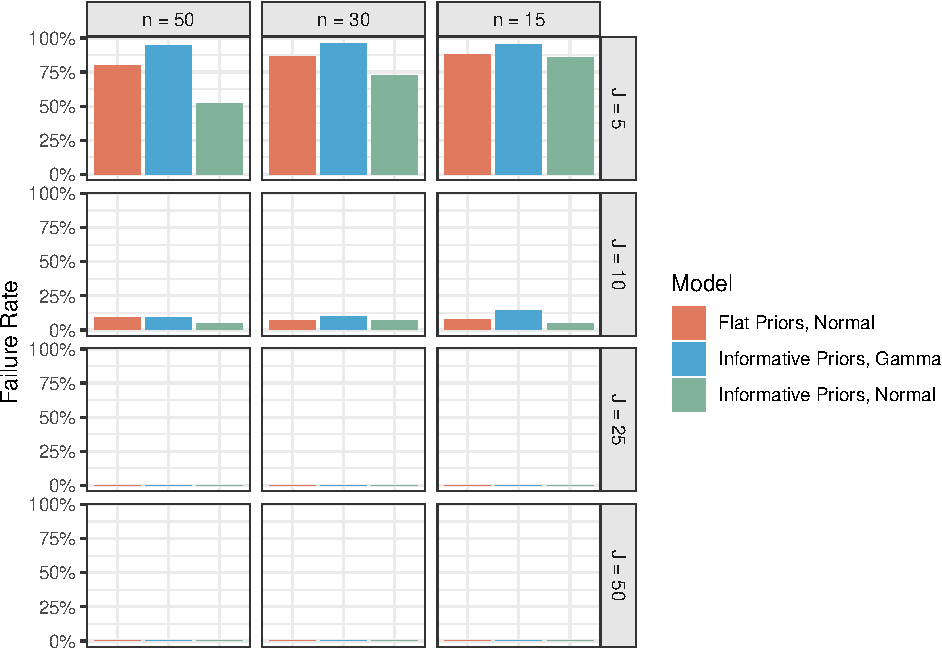
\includegraphics[width=0.85\linewidth]{thesis_files/figure-latex/failures-1} 

}

\caption{Model Failure rates across all simulation settings.}\label{fig:failures}
\end{figure}
Perhaps the most notable takeaway from Figure \ref{fig:failures} is that the number of groups that seems to drive failure rates much more than the number of observations per group. Moreover there is a massive jump in model failure rates from \(J = 10\) to \(J = 5\) that is quite alarming.

What's more, in order to avoid biasing our results, whenever we evaluate some of the models we only do so across simulation reps in which none of the models that we are comparing failed. For example, if we wanted to compare all 4 of the different models using the truncated results in the table below we might be tempted to simply remove individual rows in which the model failed. But doing so would mean that each model would be evaluated on a different number of results. To avoid this issue, we simply disregard all results from Simulation Rep 1 and only use Simulation Reps where none of the models failed (e.g Simulation Rep 2).
\begin{figure}

{\centering 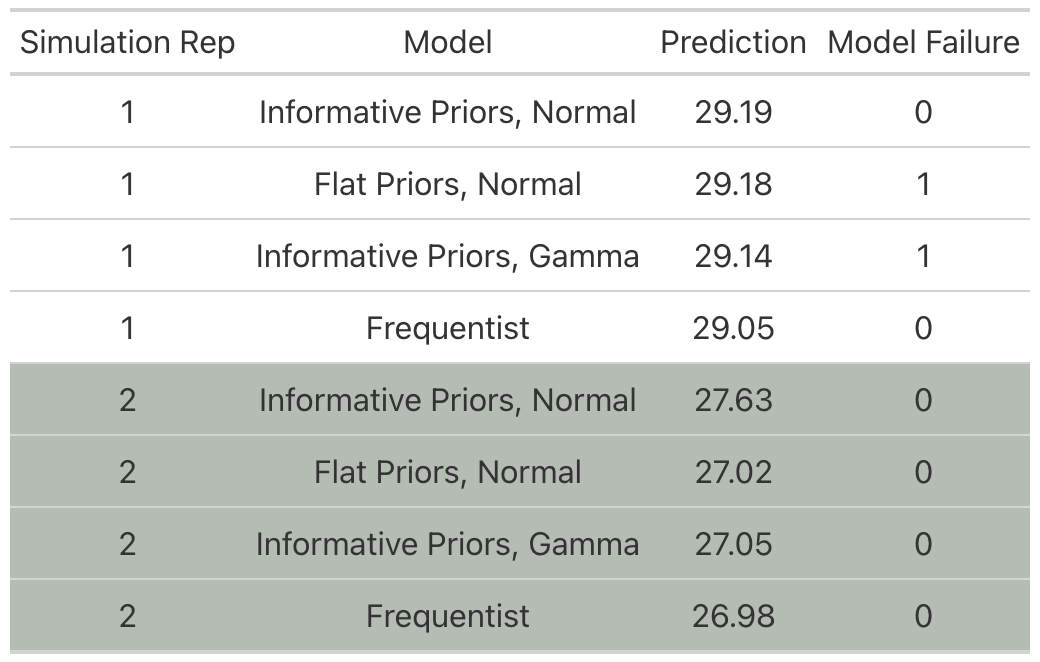
\includegraphics[width=0.95\linewidth]{figure/tb1} 

}

\caption{Results Excerpt Example}\label{fig:tbl}
\end{figure}
Of course this means that the individual model failure rates have a large impact on how much of the simulation results we are able to utilize. Below, we show what percent of the simulation results we'd be able to retain in each setting.
\begin{figure}

{\centering 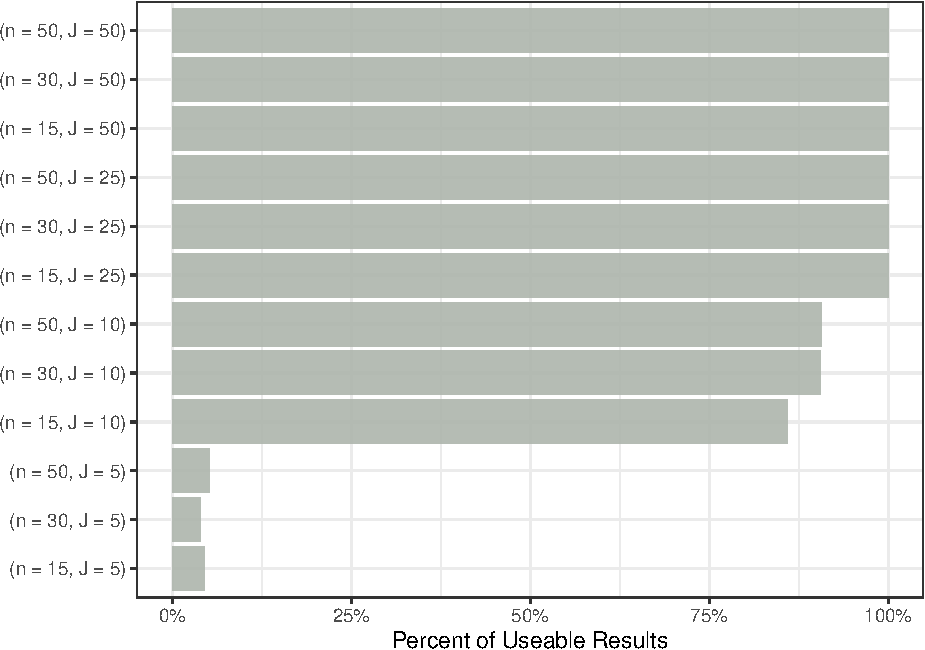
\includegraphics[width=0.85\linewidth]{thesis_files/figure-latex/keep-1} 

}

\caption{Percent of Results we would get to use if we only included simulation iterations where none of the models failed.}\label{fig:keep}
\end{figure}
Clearly the Bayesian models fail far too much for any trustworthy and meaningful conclusions to be made in any of the \(g = 5\) settings and so they will essentially be omited from the rest of the evaluation. While this may seem very disappointing, there is still an interesting takeaway that can be extracted from the high failure rates in those settings.

\hypertarget{model-regularization-through-informative-priors}{%
\subsection{Model Regularization through Informative Priors}\label{model-regularization-through-informative-priors}}

If we only compare the ``Flat Priors, Normal'' and ``Informative Priors, Normal'' failure rates, we are able to get a sense for the role that the prior distributions play here. After all these are the same underlying models just with different priors, and so their failure rates give us good insight into the power of priors to stabilize and regularize models.
\begin{figure}

{\centering 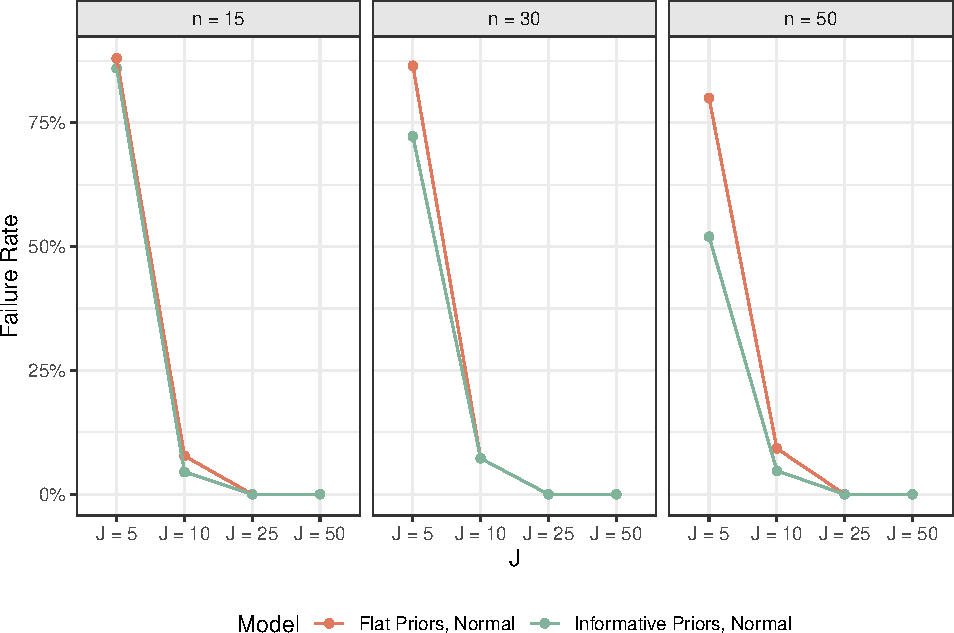
\includegraphics[width=0.85\linewidth]{thesis_files/figure-latex/regularization-1} 

}

\caption{Model Failure Rate comparison between the Bayesian Normal model with flat priors and with informative priors.}\label{fig:regularization}
\end{figure}
While in the \(J = 25\) and \(J = 50\) settings both models exhibit no failures, we do indeed see that in the smaller settings where \(J = 5\) and \(J = 10\) the model with informative priors does have lower failure rates than the model with flat priors. While informative priors do not completely ameliorate the model failure issues, it's clear that they do have a positive impact on how often a Bayesian model converges. Although we aren't saying anything about the actual performance metrics of the models here, a Bayesian model that does not converge is a model that cannot be used. This is not to say that one should always use informative priors in every Bayesian analysis setting, in fact sometimes you have no prior knowledge to employ. Rather, the lesson here should be that if you are experiencing model convergence issues in a Bayesian analysis setting, one potential fix could be to add more information into your priors.

\hypertarget{root-mean-squared-error}{%
\section{Root Mean Squared Error}\label{root-mean-squared-error}}

We begin by comparing the RMSE of our models. As a reminder, due to the high model failure rates, the settings with \(g = 5\) are not included in theses evaluations. The performance metrics below are calculated over the simulation reps in which none of the models being evaluated failed to converge (although this is only drops results in the settings where \(g = 10\) since we observed no model failures at larger values of \(g\)).
\begin{figure}

{\centering 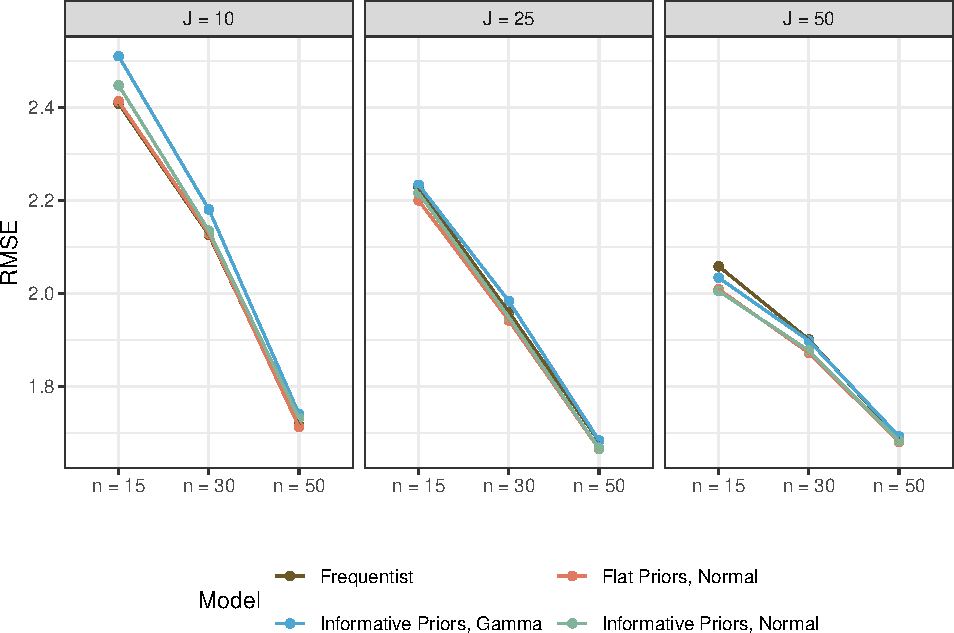
\includegraphics[width=0.85\linewidth]{thesis_files/figure-latex/rmse-1} 

}

\caption{Root Mean Squared Error}\label{fig:rmse}
\end{figure}
As we'd expect, we see decreases in RMSE across all models as the number of observations per group and the number of groups increases. Essentially as the model has access to more data, we'd expect it to be able to ``learn'' the data structure better and thus have lower prediction error. We also see that the models that consistently have some of the lowest RMSE are the Bayesian Normal model with flat priors and the Bayesian Normal model with informative priors.The only setting in which they are outperformed is when \(g = 10\) where they are marginally outperformed by the frequentist model. Note that the true value of the response for group one was \(23.7\) which gives a sense of scale for this model prediction error metric. While there are small differences in how the models performed, the differences are pretty marginal given the scale of our response.

\hypertarget{empirical-variance}{%
\section{Empirical Variance}\label{empirical-variance}}

Next we look at the empirical variance which gives a sense for how variable the predictions of the various models were across the different data sets in each simulation run.
\begin{figure}

{\centering 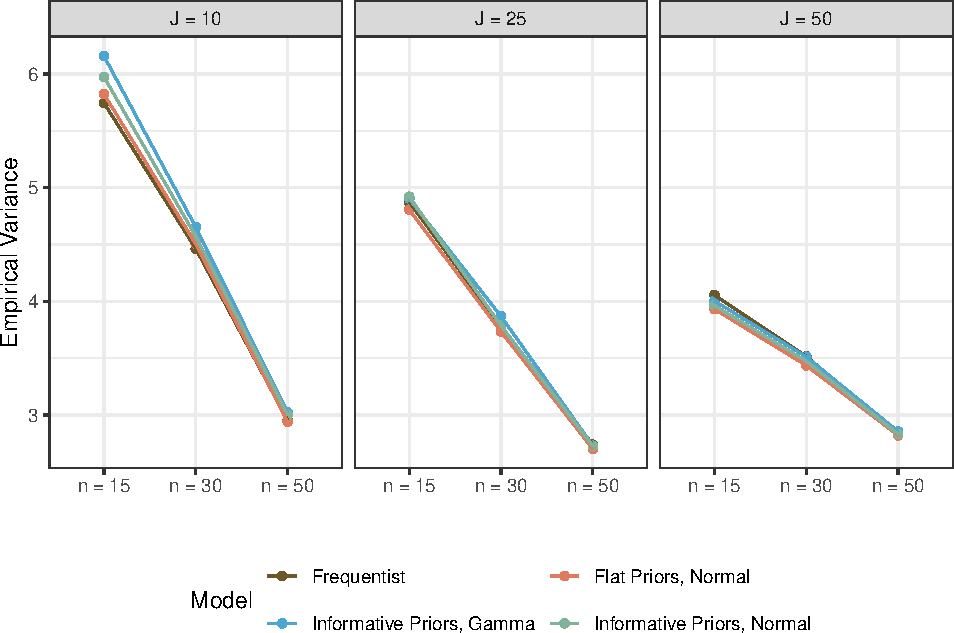
\includegraphics[width=0.85\linewidth]{thesis_files/figure-latex/variance-1} 

}

\caption{Empirical Variance}\label{fig:variance}
\end{figure}
Again we see the decrease in variance as \(n\) and \(J\) increase that we'd expect to see. And besides small amounts of separation between the models in the setting \((n = 15, \ J = 10)\), they all seem to perform very similarly.

\hypertarget{empirical-bias}{%
\section{Empirical Bias}\label{empirical-bias}}

Next we examine the Empirical Bias of the same three models. These results are by far the most unexpected as we do not see clear decreases in bias as \(n\) and \(J\) increase:
\begin{figure}

{\centering 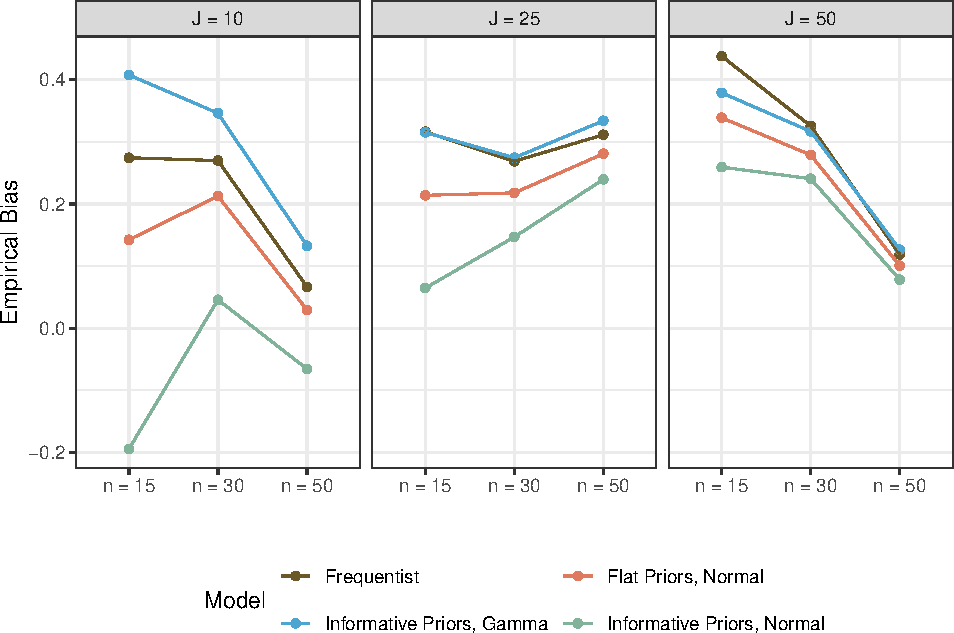
\includegraphics[width=0.85\linewidth]{thesis_files/figure-latex/bias-1} 

}

\caption{Empirical Bias}\label{fig:bias}
\end{figure}
That being said, we do see that the the Bayesian Normal model with informative priors seems to consistently have the lowest bias, with the Bayesian Normal model with flat priors performing next best. These two models perform more similarly than it may initially seem in the settings where \(g = 10\) due to the fact that the Bayesian Normal model with informative priors actually has negative bias in some of those settings. If we looked at the absolute empirical bias we would see that they perform very similarly there. Finally, even though we do see lower bias for the two Bayesian Normal models, note that the scale on the y-axis of these plots is very small. I truly wish that I could take this plot and proclaim the Bayesian Normal model with informative priors to perform far and away the best in terms of bias, but the reality is that the scale of the bias is so small for each model that there really isn't much here. In fact, it's likely this small scale that gives us the patterns that were initially a bit befuddling in Figure \ref{fig:bias}.

\hypertarget{coverage}{%
\section{Coverage}\label{coverage}}

And finally, we examine the coverage of the Bayesian models. Note that we do not include the Frequentist model here.
\begin{center}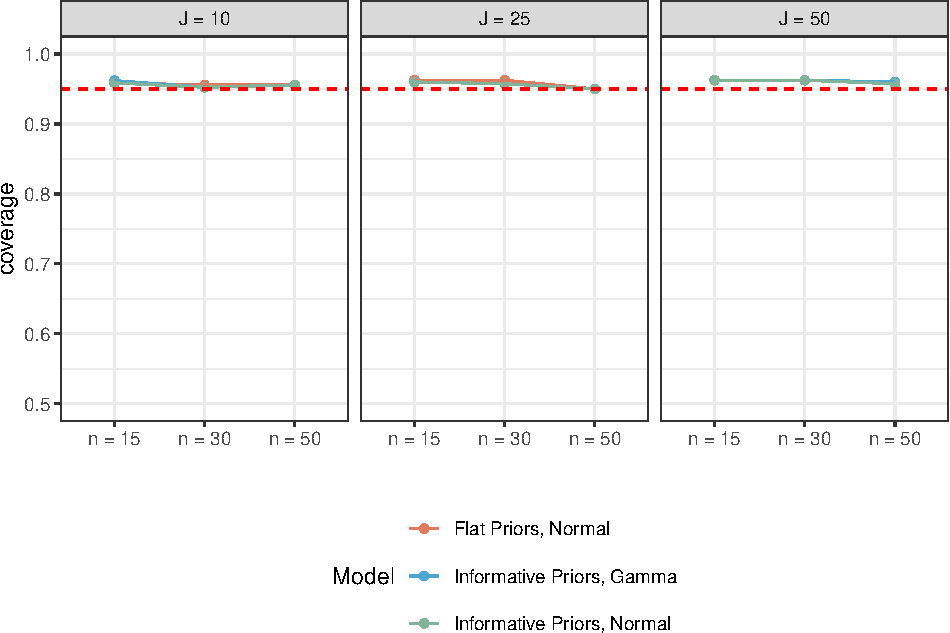
\includegraphics[width=0.85\linewidth]{thesis_files/figure-latex/unnamed-chunk-15-1} \end{center}

Interestingly, while we get close to 95\% coverage in all of our Bayesian models, we do see consistent slight over-coverage in almost every setting. While there are a certainly a couple of different reasons why this might have happened, the most prominent one in my mind has to do with the fact that the Bayesian models should all be a little bit misspecified due to the fact that the parameters in the data generating process were fixed constants. While we didn't end up seeing significant differences in bias due to this misspecification, we do see slight overcoverage as a result of it.

\hypertarget{conc}{%
\chapter{Discussion}\label{conc}}

It would be relatively easy to look at the results from Chapter \ref{res-sec} and conclude that the Bayesian model isn't really worth our time. After all, the best-performing Bayesian model in each setting performs practically identically to the Frequentist model while requiring a lot more computational work to get there. It's certainly tempting to base our conclusions solely on some of the performance metrics that we procured, but to proceed in this way would be to forget the whole point of this thesis. Recall that the point was not to go through all this work to be able to appoint either the Bayesian models or Frequentist models as being the better of the two approaches. Rather we were primarily interested in learning about Bayesian models and looking to understand when and how they are useful.

It is unfortunate that the general statistical modeling discourse is so overwhelmingly focused on performance that pedagogy and intuition for a method often take a backseat to a dense results section. There's no denying that results are important and should be presented, but problems arise when results are taken to be the only expression of a model's value. To try to break out of this mold I will walk through some takeaways from the results themselves, but I will also talk more generally about the value and usefulness of the Bayesian models that exist outside of their performance metrics.

\hypertarget{general-results-remarks}{%
\section{General Results Remarks}\label{general-results-remarks}}

As stated previously, in terms of metrics like RMSE, empirical bias, and empirical variance, most of the models that we employed performed relatively similarly. If we were approaching these simulation results with the goal of finding a method that was better than all the rest, this would be a pretty disappointing result. Luckily, we're not doing that and instead can appreciate the fact that the Bayesian and Frequentist methods, while very different in their approaches to, and conceptualizations of, the problem, ended up producing very similar results.

Perhaps the main worry when looking at the performance of the Bayesian model has to do with the model failures metric. After all, the Frequentist model never failed in any settings, while the failure rates of the Bayesian models in the \(J=5\) settings were so high that they rendered the results unuseable. I'll push back on this a little bit as a segway into the next portion of our discussion.

There's certainly an argument to be made that Bayesian model convergence failures are a good safeguard against building bad models. What I mean by this is that in some cases if your Bayesian model is not properly specified or has another substantive problem with it's formulation it will fail to converge and leave you without a useable model. I want to stress that I am not generalizing this to all cases, but in some cases this is actually good behavior because it forces you to think about what your data looks like and why your model is failing to fit to it. The Frequentist models are often so robust that it takes a very serious specification problem for them to ever fail. The main point is this: having a model that never fails is not always a good thing when trying to build a good model. To make sense of why this is, we'll look at the RMSE of the Frequentist model in the \(J = 5\) settings from our simulation in Chapter \ref{sim-study}. Recall that the Bayesian models struggled so much in these settings they had to be dropped entirely. Thus the argument could be made that the Frequentist models are better in these settings due to the fact that they never failed.
\begin{figure}

{\centering 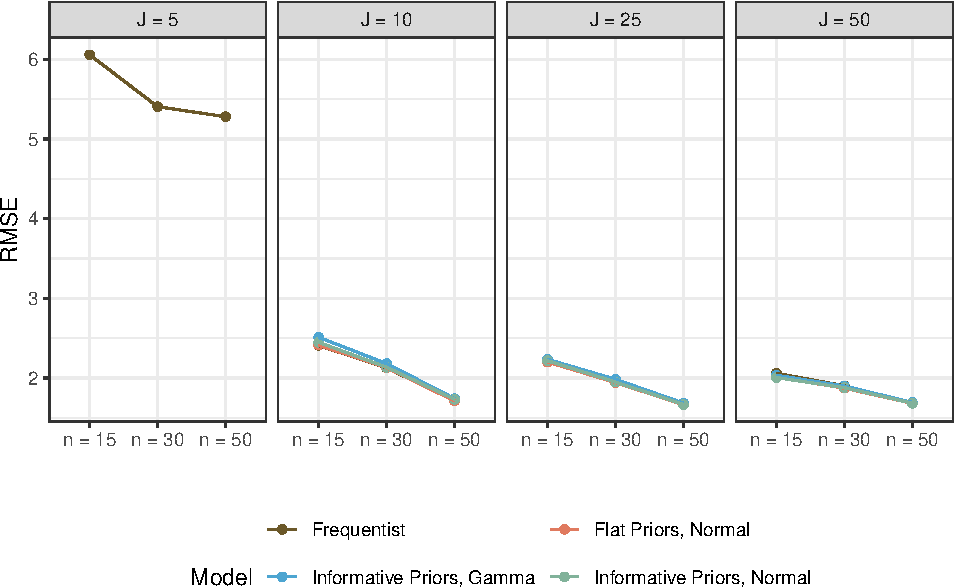
\includegraphics[width=0.85\linewidth]{thesis_files/figure-latex/j5res-1} 

}

\caption{Struggles for the Frequentist model in J = 5}\label{fig:j5res}
\end{figure}
Clearly, Figure \ref{fig:j5res} gives us plenty of reason to worry about proceeding in this way. While the Frequentist model did not fail to converge, it clearly struggled mightily in those settings. Importantly, this is not a knock against Frequentist models in \emph{all} modeling settings, but rather that in this situation it actually is advantageous that the Bayesian models are more sensitive to poor model specification.

This leads us nicely into a larger point about the ways in which Bayesian modeling as a procedure encourages intentionality and understanding.

\hypertarget{general-procedural-remarks}{%
\section{General Procedural Remarks}\label{general-procedural-remarks}}

One big barrier to Bayesian models is the added computational work involved with MCMC and the general software that exists for these methods. I won't sugar coat this part, MCMC is hard and writing code for Bayesian models in \texttt{Stan} is a laborious process. There have been enormous advances in computing that have made this aspect of Bayesian modeling more approachable, but for a general modeler, debugging MCMC problems is a real struggle. The one spin here is that with all of that additional computational work, come variance estimates and prediction intervals at no extra cost. Though recall that these variance estimates are only correct when the Bayesian models are correctly specified. That being said, regardless of how interesting and useful Bayesian modeling is, the computational burden will likely continue to keep people from utilizing it. Even with packages like \texttt{rstanarm} and \texttt{R2WinBUGS} which really streamline the process, I certainly want to acknowledge that this aspect of Bayesian modeling is still a sizeable barrier to entry.

Another way in which Bayesian models are perhaps more unattractive has to do with the procedural and conceptual load associated with building them. While I agree that computational burden is a downside of the current state of Bayesian modeling, I want to push back on the idea that this extra conceptual load is as well. Through the process of learning about Bayesian data analysis and in particular Bayesian modeling, I came to realize the ways in which the workflows can really be conducive to understanding your data and your problem more fully. For example, in order to attach informative priors to your model parameters you have to really understand where that parameter value might lie and how it might vary. Even though these decisions make the Bayesian modelling process a slower one, I ultimately think the effect is net positive, due to the fact that you are required to intuit connections between the data and the model. Of course, in larger sample size settings the prior distribution tends to have less of an effect on the model and so it can be reasonable to choose priors that are more uninformative. But even in these settings you have to restrict your priors to the range of values that your parameters could possibly take on, which requires some understanding of that connection between data and model. It's true that there's something very nice about just throwing a model formula into the \texttt{lm} function in R and getting a reasonable output, but it can sometimes become to easy to just default to using that simple linear regression without thinking about why you're doing it or if it's justified. In my mind, the extra conceptual work required by Bayesian models adds value in that it can lead to greater intentionality in model building decisions.

Hopefully these points have shed light on the ways that Bayesian models has value outside of their performance metrics. Ultimately, the goal for any data analysis methodology is to learn from data. Bayesian methods, models, and conceptualizations do just that and hopefully I've made it clear that they are interesting and valuable beyond the results that they produce.

\hypertarget{vignette}{%
\chapter{Package Vignette}\label{vignette}}

\hypertarget{forestry-data}{%
\section{Forestry Data}\label{forestry-data}}

In order to show off the functionality of the package that we wrote, we'll apply it to the Forestry data that we introduced all the way back in Chapter \ref{intro-section}. Recall that this forestry data is both zero-inflated and clustered making it a perfect setting for us to employ our models.

The particular subset of Forestry data that we'll be looking at comes from the State of Washington and contains 6960 observations across 49 Eco-Subsections (which define our clusters). The summary statistics of the number of observations per group are as follows:
\begin{verbatim}
   Min. 1st Qu.  Median    Mean 3rd Qu.    Max. 
      9      43      88     142     188     544 
\end{verbatim}
The covariate that we will be using from the forestry data is called ``Tree Canopy Cover'' (tcc) which is defined as the proportion of forest floor covered by a vertical projection of the tree crowns \footnote{Toney, Shaw, \& Nelson (2008)}. This is one of the FIA's remote sensed variables, so the information is associated with the pixels that overlay the individual plot.

The response variable that we will be using is called ``Dry Above Ground Biomass from Live Trees'' and is expressed in the units of per area density. This Dry Above Ground Biomass variable is one that is very important for understanding the health of forest ecosystems and plays a role in decisions regarding merchantable timber and fire hazard. For these reasons its vitally important for the FIA to be able to produce accurate estimates of this variable.

The zero-inflation models presented in this thesis provide a reasonable approach for trying to do exactly that. That being said, no matter how good a method is, it can't be used if the tooling doesn't exist to actually perform it. Thus, the last portion of this thesis will be devoted to describing the very early stages of an R software package that we have written to build and utilize these zero-inflation models.

\hypertarget{r-package-zinf}{%
\section{R Package: zinf}\label{r-package-zinf}}

We start by installing the developmental version of the package and loading it into our R session.
\begin{Shaded}
\begin{Highlighting}[]
\NormalTok{devtools}\SpecialCharTok{::}\FunctionTok{install\_github}\NormalTok{(}\StringTok{"joshyam{-}k/zinf"}\NormalTok{)}
\FunctionTok{library}\NormalTok{(zinf)}
\end{Highlighting}
\end{Shaded}
The two main functions that \texttt{zinf} contains are \texttt{zinf\_bayes} and \texttt{zinf\_freq} which as the names suggest relate to the Frequentist and Bayesian versions of the zero-inflation models.

The challenge of writing a software package for these zero-inflation models was truthfully a lot trickier than I initially thought it would be. There were two different possible structural versions that I considered to be viable:
\begin{enumerate}
\def\labelenumi{\arabic{enumi}.}
\tightlist
\item
  Write a function that takes as argument all the individual pieces needed to build each of the two models and internally build the two models and then define all of the neccessary functionality.
\item
  Write a function that takes as argument each of the two already built models and internally combine the models into a single object and define all of the neccessary functionality.
\end{enumerate}
On the one hand, version (1) is nice in that it ``does it all'' for the user. But the main problem with version (1) is that the functions \texttt{lme4::lmer} and \texttt{lme4::glmer} for Frequentist models and \texttt{rstanarm::stan\_lmer} and \texttt{rstanarm::stan\_glmer} for Bayesian models are already so popular and well developed and robust that it seems silly to to rely on that pre-existing software. After all, as we showed in Section \ref{sepsim}, the Bayesian models can be built separately and made as complex desired, and this is also certainly the case for the Frequentist models. So, while there's an argument to be made for the abstraction of all model building processes, the reality is that under version (1) if I wanted my package to be as familiar and robust as the pre-existing software for building the individual models, I would have to essentially take as arguments every possible function arguments that those \texttt{lme4} and \texttt{rstanarm} functions take, and internally feed them back into those functions. At that point the question becomes: why not just have the user build the individual models separately and then feed those finished models into our function? And that lands us directly at version (2).
\begin{figure}

{\centering 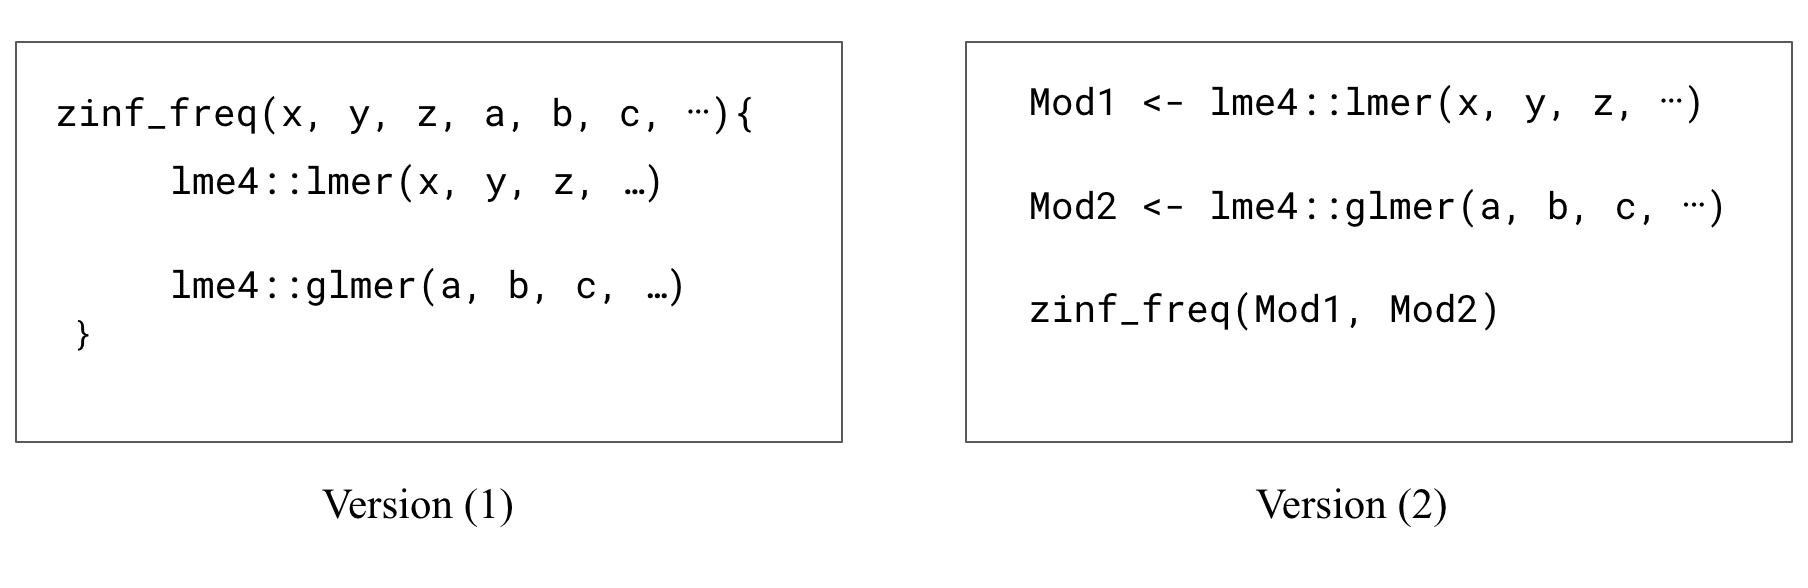
\includegraphics[width=0.9\linewidth]{figure/v1v2} 

}

\caption{Two Software Versions}\label{fig:tbl2}
\end{figure}
In the Frequentist setting, version (1) doesn't seem that bad, especially since most of the time a user only specifies the model formula and the data set within the \texttt{lme4} functions, but things grow a lot worse in the bayesian versions where all kinds of priors and MCMC settings need to be specified. In the end, I decided that it made more sense to build version (2). While this does leave more work for the user than I would have liked, I think that the \texttt{zinf} functions still have enormous usefullness in that they define methods for producing a summary of the zero-inflation model and most importantly for predicting with the zero-inflation model.

\hypertarget{application}{%
\section{Application}\label{application}}

We'll start by setting aside a small amount of the data set to make predictions on. In particular, Ecosubsections M242Ba and M242Db have quite a few data points so we'll sample 100 points from each one to test our model on. The only other data preparation we need to do is to create a training data set that only contains training data points with a non-zero response value.
\begin{Shaded}
\begin{Highlighting}[]
\FunctionTok{set.seed}\NormalTok{(}\DecValTok{5}\NormalTok{)}
\NormalTok{test }\OtherTok{\textless{}{-}}\NormalTok{ data }\SpecialCharTok{\%\textgreater{}\%} 
  \FunctionTok{filter}\NormalTok{(ECOSUBCD }\SpecialCharTok{\%in\%} \FunctionTok{c}\NormalTok{(}\StringTok{"M242Ba"}\NormalTok{, }\StringTok{"M242Db"}\NormalTok{)) }\SpecialCharTok{\%\textgreater{}\%} 
  \FunctionTok{group\_by}\NormalTok{(ECOSUBCD) }\SpecialCharTok{\%\textgreater{}\%} 
  \FunctionTok{slice\_sample}\NormalTok{(}\AttributeTok{n =} \DecValTok{100}\NormalTok{) }\SpecialCharTok{\%\textgreater{}\%} 
  \FunctionTok{ungroup}\NormalTok{()}

\NormalTok{train }\OtherTok{\textless{}{-}} \FunctionTok{anti\_join}\NormalTok{(data, test)}

\NormalTok{nonzero\_train }\OtherTok{\textless{}{-}}\NormalTok{ train }\SpecialCharTok{\%\textgreater{}\%} 
  \FunctionTok{filter}\NormalTok{(DRYBIO\_AG\_TPA\_live\_ADJ }\SpecialCharTok{\textgreater{}} \DecValTok{0}\NormalTok{)}
\end{Highlighting}
\end{Shaded}
\hypertarget{individual-frequentist-models}{%
\subsection{Individual Frequentist models}\label{individual-frequentist-models}}

We'll start by building the individual Frequentist models.
\begin{Shaded}
\begin{Highlighting}[]
\FunctionTok{library}\NormalTok{(lme4)}

\NormalTok{freq\_reg }\OtherTok{\textless{}{-}} \FunctionTok{lmer}\NormalTok{(}
\NormalTok{  DRYBIO\_AG\_TPA\_live\_ADJ }\SpecialCharTok{\textasciitilde{}}\NormalTok{ tcc }\SpecialCharTok{+}\NormalTok{ (}\DecValTok{1} \SpecialCharTok{|}\NormalTok{ ECOSUBCD),}
  \AttributeTok{data =}\NormalTok{ nonzero\_train}
\NormalTok{  )}

\NormalTok{freq\_log\_reg }\OtherTok{\textless{}{-}} \FunctionTok{glmer}\NormalTok{(}
\NormalTok{  DRYBIO\_AG\_TPA\_live\_ADJ }\SpecialCharTok{!=} \DecValTok{0} \SpecialCharTok{\textasciitilde{}}\NormalTok{ tcc }\SpecialCharTok{+}\NormalTok{ (}\DecValTok{1} \SpecialCharTok{|}\NormalTok{ ECOSUBCD),}
  \AttributeTok{family =}\NormalTok{ binomial,}
  \AttributeTok{data =}\NormalTok{ train}
\NormalTok{  )}
\end{Highlighting}
\end{Shaded}
The key characteristics of these models are the specification of the covariates and the response, the random intercept term for the Ecosubsection (ECOSUBCD), and the use of the non-zero data set to fit the first model.

\hypertarget{individual-bayesian-models}{%
\subsection{Individual bayesian models}\label{individual-bayesian-models}}

\hypertarget{logistic-regression-model}{%
\subsubsection{Logistic Regression Model}\label{logistic-regression-model}}

Next we'll build the individual Bayesian models. We'll start with the logistic regression model that requires priors for
\begin{itemize}
\tightlist
\item
  The fixed effect slope (for tcc)
\item
  The fixed effect intercept
\item
  The variance of the random intercepts
\end{itemize}
The prior fixed effect slope should reflect our vague sense for how the probability of Dry Above Ground Biomass from Live Trees being non-zero changes with Tree Canopy Cover. With limited knowledge of how forest attributes interact we'll assume that the slope is positive and centered somewhere around 0.5, so we'll use a prior of \(\mathcal{N}(0.5, 0.25^2)\).

The fixed effect intercept that \texttt{rstanarm::stan\_glmer} asks for is actually the centered intercept. This can be conceptualized as our guess for the probability of being non-zero for an average plot. Given that the response variable is zero in around 40\% of the plots in our data set we'll guess that this probability is around 0.4. We have to be careful here, since logistic regression employs a logit link, we actually want to set the prior mean to be on the log-odds scale, so we use \(\log{(0.4/(1-0.4))} = -0.4\) as the center. We might guess that the range of the propbability of being non-zero for an average plot might range from 0.1 to 0.7 which translates to a log odds range of \((-2.2, 0.85)\). Thus the prior for the centered fixed effect intercept will thus be \(\mathcal{N}(-0.4, 0.7^2)\).

Finally, the variance of the random intercepts is not really a parameter that we can use the data to get a great guess for, so we'll utilize a weakly informative prior of Exponential\((1)\). In \texttt{rstanarm::stan\_glmer} this is written slightly differently using a function called \texttt{decov} but in this setting that is just the Exponential\((1)\) prior that we want.

We'll stick with the default MCMC settings and build the model as follows
\begin{Shaded}
\begin{Highlighting}[]
\FunctionTok{library}\NormalTok{(rstanarm)}
\NormalTok{bayes\_log\_reg }\OtherTok{\textless{}{-}} \FunctionTok{stan\_glmer}\NormalTok{(}
\NormalTok{  DRYBIO\_AG\_TPA\_live\_ADJ }\SpecialCharTok{\textgreater{}} \DecValTok{0} \SpecialCharTok{\textasciitilde{}}\NormalTok{ tcc }\SpecialCharTok{+}\NormalTok{ (}\DecValTok{1} \SpecialCharTok{|}\NormalTok{ ECOSUBCD),}
  \AttributeTok{data =}\NormalTok{ train,}
  \AttributeTok{family =}\NormalTok{ binomial,}
  \AttributeTok{prior =} \FunctionTok{normal}\NormalTok{(}\FloatTok{0.5}\NormalTok{, }\FloatTok{0.25}\NormalTok{),}
  \AttributeTok{prior\_intercept =} \FunctionTok{normal}\NormalTok{(}\SpecialCharTok{{-}}\FloatTok{0.4}\NormalTok{, }\FloatTok{0.7}\SpecialCharTok{\^{}}\DecValTok{2}\NormalTok{),}
  \AttributeTok{prior\_covariance =} \FunctionTok{decov}\NormalTok{(}\AttributeTok{reg =} \DecValTok{1}\NormalTok{, }\AttributeTok{conc =} \DecValTok{1}\NormalTok{, }\AttributeTok{shape =} \DecValTok{1}\NormalTok{, }\AttributeTok{scale =} \DecValTok{1}\NormalTok{),}
  \AttributeTok{chains =} \DecValTok{4}\NormalTok{, }\AttributeTok{iter =} \DecValTok{2000}\NormalTok{, }\AttributeTok{seed =} \DecValTok{84735}\NormalTok{,}
  \AttributeTok{cores =}\NormalTok{ parallel}\SpecialCharTok{::}\FunctionTok{detectCores}\NormalTok{()}
\NormalTok{)}
\end{Highlighting}
\end{Shaded}
\hypertarget{glm-1-normal-with-identity-link}{%
\subsubsection{GLM 1: Normal with Identity link}\label{glm-1-normal-with-identity-link}}

We now turn to the two versions of the generalized linear model. We'll start with the model that uses a Normal distribution and the identity link- i.e Normal linear regression. This time the parameters that need priors are all the same as from the previous one, except now we also need a prior for the variance of the error term.

We can examine a scatter plot of Tree Canopy Cover on Dry Above Ground Biomass from Live Trees to choose our prior for the fixed effect slope. We can do some rise-over-run calculations to end up with a guess that the fixed effect slope is around 2 and probably doesn't go outside of the range (0.5, 5). Thus we'll use a \(\mathcal{N}(2, 1^2)\) prior here.
\begin{figure}

{\centering 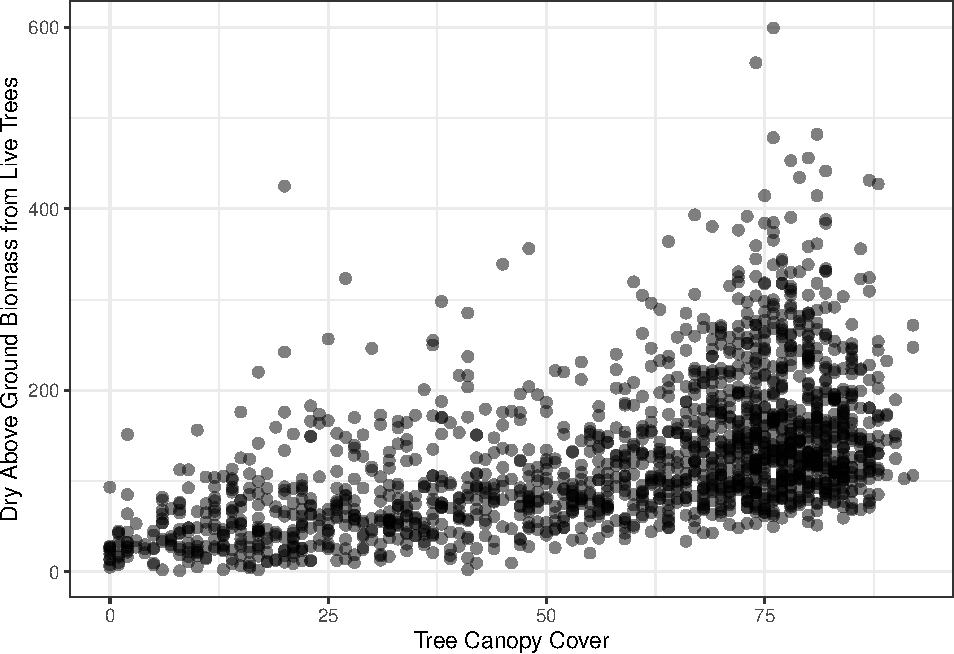
\includegraphics[width=0.9\linewidth]{thesis_files/figure-latex/nzdata-1} 

}

\caption{Relationship between Tree Canopy Cover and Dry Above Ground Biomass from Live Trees}\label{fig:nzdata}
\end{figure}
Again we can refer back to Figure \ref{fig:nzdata} to get our guess for the the centered intercept. At an average value of tcc (say 50), the value of the response looks to be around 100, but this could plausibly range anywhere between 20 and 180, so we'll use a \(\mathcal{N}(100, 40^2)\) prior for the centered intercept.

Finally we'll stick with an Exponential\((1)\) prior for the two variance parameters since we don't know enough to say more about them. We can plug all of this in to \texttt{rstanarm::stan\_lmer} as follows.
\begin{Shaded}
\begin{Highlighting}[]
\NormalTok{bayes\_normal\_reg }\OtherTok{\textless{}{-}} \FunctionTok{stan\_lmer}\NormalTok{(}
\NormalTok{  DRYBIO\_AG\_TPA\_live\_ADJ }\SpecialCharTok{\textasciitilde{}}\NormalTok{ tcc }\SpecialCharTok{+}\NormalTok{ (}\DecValTok{1} \SpecialCharTok{|}\NormalTok{ ECOSUBCD),}
  \AttributeTok{data =}\NormalTok{ nonzero\_train,}
  \AttributeTok{prior =} \FunctionTok{normal}\NormalTok{(}\DecValTok{2}\NormalTok{, }\DecValTok{1}\NormalTok{),}
  \AttributeTok{prior\_intercept =} \FunctionTok{normal}\NormalTok{(}\DecValTok{100}\NormalTok{, }\DecValTok{40}\NormalTok{),}
  \AttributeTok{prior\_aux =} \FunctionTok{exponential}\NormalTok{(}\DecValTok{1}\NormalTok{),}
  \AttributeTok{prior\_covariance =} \FunctionTok{decov}\NormalTok{(}\AttributeTok{reg =} \DecValTok{1}\NormalTok{, }\AttributeTok{conc =} \DecValTok{1}\NormalTok{, }\AttributeTok{shape =} \DecValTok{1}\NormalTok{, }\AttributeTok{scale =} \DecValTok{1}\NormalTok{),}
  \AttributeTok{chains =} \DecValTok{4}\NormalTok{, }\AttributeTok{iter =} \DecValTok{2000}\NormalTok{, }\AttributeTok{seed =} \DecValTok{84735}\NormalTok{,}
  \AttributeTok{cores =}\NormalTok{ parallel}\SpecialCharTok{::}\FunctionTok{detectCores}\NormalTok{()}
\NormalTok{)}
\end{Highlighting}
\end{Shaded}
\hypertarget{glm-2-gamma-with-log-link}{%
\subsubsection{GLM 2: Gamma with log link}\label{glm-2-gamma-with-log-link}}

We'll stick with the same priors for the fixed effects as before except we'll put all of the parameter values on a log scale due to the fact that we're using a log link function.
\begin{itemize}
\tightlist
\item
  fixed effect slope: \(\mathcal{N}(0.7, 0.1^2)\)
\item
  fixed effect intercept: \(\mathcal{N}(4.6, 3.6^2)\)
\end{itemize}
Similarly we'll keep our weakly informative prior for the variance of the random intercepts, and so all that's left is to decide what prior we should use for the shape parameter of the Gamma distribution. We'll follow the logic employed in Section \ref{info} to do this. The estimation simply relies on the fact that the mean of a Gamma\((\alpha, \beta)\) distribution is \(\alpha/\beta\) and the variance is \(\alpha/\beta^2\). Here \(\bar{y}\) and \(s^2\) represent the sample mean and variance of Dry Above Ground Biomass from Live Trees.
\begin{equation}
\bar{y} = 80.45 \approx \frac{\alpha}{\beta}\qquad \text{and} \qquad s^2 = 6029 \approx \frac{\alpha}{\beta^2}
\label{eq:first}
\end{equation}
but now,
\begin{equation}
\frac{\bar{y}}{s^2} = 0.013 \approx \frac{\alpha / \beta}{\alpha / \beta^2} = \beta 
\end{equation}
and if we put our estimate for \(\beta\) back into \eqref{eq:first} to get
\begin{equation}
\frac{\alpha}{0.013} \approx 80.45 \implies \alpha \approx 1.04
\end{equation}
We aren't positive about this guess but we know that the actuall parameter has to be non-negative so we'll use a Half-Cauchy\((1, 1)\) prior here. Note that \texttt{rstanarm::stan\_glmer} assumes all \texttt{prior\_aux} parameters are positive so we don't have to specify that it's a bounded Cauchy distribution.
\begin{Shaded}
\begin{Highlighting}[]
\NormalTok{bayes\_gamma\_reg }\OtherTok{\textless{}{-}} \FunctionTok{stan\_glmer}\NormalTok{(}
\NormalTok{  DRYBIO\_AG\_TPA\_live\_ADJ }\SpecialCharTok{\textasciitilde{}}\NormalTok{ tcc }\SpecialCharTok{+}\NormalTok{ (}\DecValTok{1} \SpecialCharTok{|}\NormalTok{ ECOSUBCD),}
  \AttributeTok{data =}\NormalTok{ nonzero\_train,}
  \AttributeTok{family =} \FunctionTok{Gamma}\NormalTok{(}\AttributeTok{link =} \StringTok{"log"}\NormalTok{),}
  \AttributeTok{prior =} \FunctionTok{normal}\NormalTok{(}\FloatTok{0.7}\NormalTok{, }\FloatTok{0.1}\NormalTok{),}
  \AttributeTok{prior\_intercept =} \FunctionTok{normal}\NormalTok{(}\FloatTok{4.6}\NormalTok{, }\FloatTok{3.6}\NormalTok{),}
  \AttributeTok{prior\_aux =} \FunctionTok{cauchy}\NormalTok{(}\DecValTok{1}\NormalTok{, }\DecValTok{1}\NormalTok{),}
  \AttributeTok{prior\_covariance =} \FunctionTok{decov}\NormalTok{(}\AttributeTok{reg =} \DecValTok{1}\NormalTok{, }\AttributeTok{conc =} \DecValTok{1}\NormalTok{, }\AttributeTok{shape =} \DecValTok{1}\NormalTok{, }\AttributeTok{scale =} \DecValTok{1}\NormalTok{),}
  \AttributeTok{chains =} \DecValTok{4}\NormalTok{, }\AttributeTok{iter =} \DecValTok{2000}\NormalTok{, }\AttributeTok{seed =} \DecValTok{84735}\NormalTok{,}
  \AttributeTok{cores =}\NormalTok{ parallel}\SpecialCharTok{::}\FunctionTok{detectCores}\NormalTok{()}
\NormalTok{)}
\end{Highlighting}
\end{Shaded}
Again, just from the length of these Bayesian model building sections compared to the Frequentist sections, it's clear how much extra work is required if you want to use informative priors. That being said, I hope it's clear how going through this process does force you to understand the dynamics of the data and know how to connect them back to the model, which in my mind is a very positive thing.

\hypertarget{using-zinf}{%
\subsection{Using zinf}\label{using-zinf}}

In order to turn our individual models into a zero-inflation model we simply feed them into the appropriate \texttt{zinf\_*} function.
\begin{Shaded}
\begin{Highlighting}[]
\NormalTok{frequentist\_zi\_mod }\OtherTok{\textless{}{-}} \FunctionTok{zinf\_freq}\NormalTok{(freq\_reg, freq\_log\_reg)}
\NormalTok{bayesian\_zi\_mod\_normal }\OtherTok{\textless{}{-}} \FunctionTok{zinf\_bayes}\NormalTok{(bayes\_normal\_reg, bayes\_log\_reg)}
\NormalTok{bayesian\_zi\_mod\_gamma }\OtherTok{\textless{}{-}} \FunctionTok{zinf\_bayes}\NormalTok{(bayes\_gamma\_reg, bayes\_log\_reg)}
\end{Highlighting}
\end{Shaded}
If we examine the class of these objects we'll find that they're of class \texttt{zinf\_freq} and \texttt{zinf\_bayes} respectively.
\begin{Shaded}
\begin{Highlighting}[]
\FunctionTok{class}\NormalTok{(frequentist\_zi\_mod)}
\end{Highlighting}
\end{Shaded}
\begin{verbatim}
[1] "zinf_freq"
\end{verbatim}
\begin{Shaded}
\begin{Highlighting}[]
\FunctionTok{class}\NormalTok{(bayesian\_zi\_mod\_normal)}
\end{Highlighting}
\end{Shaded}
\begin{verbatim}
[1] "zinf_bayes"
\end{verbatim}
At first this might not seem like much, but the real usefulness of the software package lies in the fact that it defines \texttt{zinf\_bayes} and \texttt{zinf\_freq} as S3 generics. In R ``the job of an S3 generic is to perform method dispatch, i.e.~find the specific implementation for a class.''\footnote{Wickham (2019)}. So what \texttt{zinf} is really doing is defining methods like \texttt{predict()} and \texttt{summary()} for these zero-inflation model objects. The upshot is that we can now use these model objects much in the same way as we do for typical model objects in R.

And as we can see below, making predictions on the test dataset using our Frequentist zero-inflation model is a very familiar process. Since the estimand we're interested in is the Ecosubsection level mean and our test data set included two Ecosubsections, we get an output with two rows.
\begin{Shaded}
\begin{Highlighting}[]
\FunctionTok{predict}\NormalTok{(frequentist\_zi\_mod, }\AttributeTok{newdata =}\NormalTok{ test)}
\end{Highlighting}
\end{Shaded}
\begin{verbatim}
# A tibble: 2 x 2
  ECOSUBCD prediction
  <chr>         <dbl>
1 M242Ba         88.5
2 M242Db         71.0
\end{verbatim}
While the output will look slightly different for the Bayesian model, the process of getting the predictions is exactly the same. We'll start by looking at the Bayesian model where the GLM component assumes a Normal response
\begin{Shaded}
\begin{Highlighting}[]
\NormalTok{bayes\_preds\_normal }\OtherTok{\textless{}{-}} \FunctionTok{predict}\NormalTok{(bayesian\_zi\_mod\_normal, }\AttributeTok{newdata =}\NormalTok{ test)}
\end{Highlighting}
\end{Shaded}
The object returned by running \texttt{predict} on one of the Bayesian zero-inflation models is a list that contains two items:
\begin{itemize}
\tightlist
\item
  A data frame containing the group level predictions which in this case are the centers of the posterior predictive distributions for each group
\item
  A data frame containing the raw posterior predictive distributions for each group
\end{itemize}
If we examine the first item we see a very similar result to that of the direct output of the Frequentist predictions, except now we also have upper and lower bounds for 95\% prediction intervals.
\begin{Shaded}
\begin{Highlighting}[]
\NormalTok{bayes\_preds\_normal}\SpecialCharTok{$}\NormalTok{posterior\_predictive\_centers}
\end{Highlighting}
\end{Shaded}
\begin{verbatim}
   group post_pred_centers    lower     upper
1 M242Ba          88.41021 73.39606 102.72571
2 M242Db          71.04143 56.44706  85.59905
\end{verbatim}
But since Bayesian predictions are distributions themselves, you can access the raw distributions as follows. We'll just look at the first five rows of this data frame to get an idea of what it looks like.
\begin{Shaded}
\begin{Highlighting}[]
\NormalTok{bayes\_preds\_normal}\SpecialCharTok{$}\NormalTok{posterior\_predictive\_distribution }\SpecialCharTok{\%\textgreater{}\%} 
  \FunctionTok{head}\NormalTok{(}\DecValTok{5}\NormalTok{) }
\end{Highlighting}
\end{Shaded}
\begin{verbatim}
# A tibble: 5 x 2
      x group 
  <dbl> <chr> 
1  81.1 M242Ba
2  89.6 M242Ba
3  90.5 M242Ba
4  86.4 M242Ba
5  75.5 M242Ba
\end{verbatim}
With this we can actually plot the posterior predictive distributions for each group.
\begin{Shaded}
\begin{Highlighting}[]
\NormalTok{bayes\_preds\_normal}\SpecialCharTok{$}\NormalTok{posterior\_predictive\_distribution }\SpecialCharTok{\%\textgreater{}\%} 
  \FunctionTok{ggplot}\NormalTok{(}\FunctionTok{aes}\NormalTok{(}\AttributeTok{x =}\NormalTok{ x, }\AttributeTok{fill =}\NormalTok{ group)) }\SpecialCharTok{+}
  \FunctionTok{geom\_density}\NormalTok{(}\AttributeTok{alpha =} \FloatTok{0.5}\NormalTok{, }\AttributeTok{color =} \ConstantTok{NA}\NormalTok{) }\SpecialCharTok{+}
  \FunctionTok{theme\_bw}\NormalTok{()}
\end{Highlighting}
\end{Shaded}
\begin{figure}

{\centering 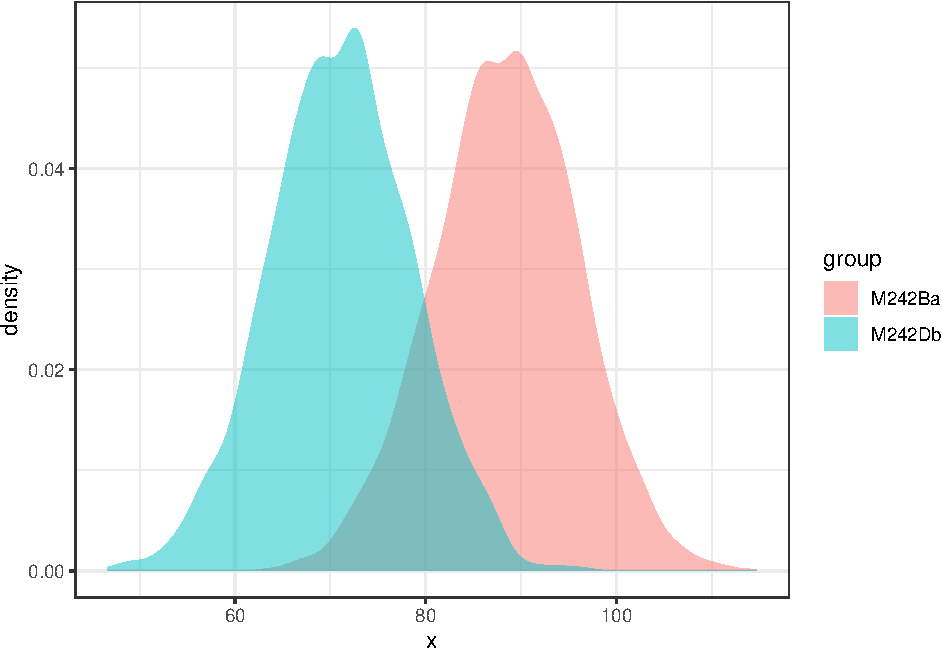
\includegraphics[width=0.85\linewidth]{thesis_files/figure-latex/unnamed-chunk-28-1} 

}

\caption{Posterior Predictive Distributions for the two groups in our test dataset}\label{fig:unnamed-chunk-28}
\end{figure}
Finally if we also compute the predictions for our Bayesian model with a Gamma GLM, then we can aggregate and look at how the models compared.
\begin{longtable}{ccccc}
\toprule
group & Bayes Gamma & Bayes Normal & Frequentist & True Mean \\ 
\midrule
M242Ba & $87.26$ & $88.41$ & $88.55$ & $95.73$ \\ 
M242Db & $68.86$ & $71.04$ & $70.99$ & $80.12$ \\ 
\bottomrule
\end{longtable}
It's nice to see that the Bayesian model where the non-zero response was modeled using a Gamma distribution performed the best, but again this is just an example about how to use the package and we shouldn't read too much into these short results.

\hypertarget{next-steps}{%
\section{Next Steps}\label{next-steps}}

Right now the package is fairly limited in that it can primarily only deal with the models that we worked with in this thesis, so there's plenty of work to be done in that regard. Moreover, while zero-inflated data are fairly common, zero-inflated clustered data are much less common, so a good extension would be to extend the package to work with models without random effects. That being said, I still believe that the package is enormously useful as is. In particular Bayesian prediction is an incredibly cumbersome task to do on your own, and it's even more difficult in this two-part model setting. Thus, having a package like \texttt{zinf} that will abstract away a lot of that messy process contributes a lot to the field of research surrounding these zero-inflation models.

\backmatter

\hypertarget{references}{%
\chapter*{References}\label{references}}
\addcontentsline{toc}{chapter}{References}

\markboth{References}{References}

\noindent

\setlength{\parindent}{-0.20in}

\hypertarget{refs}{}
\begin{CSLReferences}{1}{0}
\leavevmode\vadjust pre{\hypertarget{ref-chandra2012small}{}}%
Chandra, H., \& Sud, U. (2012). Small area estimation for zero-inflated data. \emph{Communications in Statistics-Simulation and Computation}, \emph{41}(5), 632--643.

\leavevmode\vadjust pre{\hypertarget{ref-datta1991bayesian}{}}%
Datta, G. S., \& Ghosh, M. (1991). Bayesian prediction in linear models: Applications to small area estimation. \emph{The Annals of Statistics}, 1748--1770.

\leavevmode\vadjust pre{\hypertarget{ref-dreassi2014small}{}}%
Dreassi, E., Petrucci, A., \& Rocco, E. (2014). Small area estimation for semicontinuous skewed spatial data: An application to the grape wine production in tuscany. \emph{Biometrical Journal}, \emph{56}(1), 141--156.

\leavevmode\vadjust pre{\hypertarget{ref-gelman2006prior}{}}%
Gelman, A. (2006). Prior distributions for variance parameters in hierarchical models (comment on article by browne and draper).

\leavevmode\vadjust pre{\hypertarget{ref-gelman1995bayesian}{}}%
Gelman, A., Carlin, J. B., Stern, H. S., \& Rubin, D. B. (1995). \emph{Bayesian data analysis}. Chapman; Hall/CRC.

\leavevmode\vadjust pre{\hypertarget{ref-gelman2006data}{}}%
Gelman, A., \& Hill, J. (2006). \emph{Data analysis using regression and multilevel/hierarchical models}. Cambridge university press.

\leavevmode\vadjust pre{\hypertarget{ref-johnson2022bayes}{}}%
Johnson, A. A., Ott, M. Q., \& Dogucu, M. (2022). \emph{Bayes rules!: An introduction to applied bayesian modeling}. CRC Press.

\leavevmode\vadjust pre{\hypertarget{ref-krieg2016small}{}}%
Krieg, S., Boonstra, H. J., \& Smeets, M. (2016). Small-area estimation with zero-inflated data--a simulation study. \emph{Journal of Official Statistics}, \emph{32}(4), 963--986.

\leavevmode\vadjust pre{\hypertarget{ref-mcconville2020tutorial}{}}%
McConville, K. S., Moisen, G. G., \& Frescino, T. S. (2020). A tutorial on model-assisted estimation with application to forest inventory. \emph{Forests}, \emph{11}(2), 244.

\leavevmode\vadjust pre{\hypertarget{ref-pfeffermann2008small}{}}%
Pfeffermann, D., Terryn, B., \& Moura, F. A. (2008). Small area estimation under a two-part random effects model with application to estimation of literacy in developing countries. \emph{Survey Methodology}, \emph{34}(2), 235--249.

\leavevmode\vadjust pre{\hypertarget{ref-rao2015small}{}}%
Rao, J. N., \& Molina, I. (2015). \emph{Small area estimation}. John Wiley \& Sons.

\leavevmode\vadjust pre{\hypertarget{ref-toney2008stem}{}}%
Toney, C., Shaw, J. D., \& Nelson, M. D. (2008). A stem-map model for predicting tree canopy cover of forest inventory and analysis (FIA) plots. In \emph{Forest inventory and analysis symposium}.

\leavevmode\vadjust pre{\hypertarget{ref-white2021hierarchical}{}}%
White, G. W., McConville, K. S., Moisen, G. G., \& Frescino, T. S. (2021). Hierarchical bayesian small area estimation using weakly informative priors in ecologically homogeneous areas of the interior western forests. \emph{Frontiers in Forests and Global Change}, 178.

\leavevmode\vadjust pre{\hypertarget{ref-wickham2019advanced}{}}%
Wickham, H. (2019). \emph{Advanced r}. CRC press.

\end{CSLReferences}

% Index?

\end{document}
